\begin{quote}
\textit{``Where are you?'' Hiro says.
\\
\\
``In Reality or the Metaverse?''
\\
\\
``Both.''}
\end{quote}
\hfill \textit{Snow Crash, Neal Stephenson}
\\
\\

%=========================================================================================================
%=========================================================================================================

\label{chapter-background}

% 'Position' section from experimental plan document

%\section{Introduction}

The subject of this thesis is a new category of alternate reality that allows its user to observe and move around their real environment whilst also being able to view a complete alternative virtual environment from the equivalent vantage point. This combination of real and virtual environments, combined with maintained user mobility, is not fully encapsulated by any previously defined alternate reality terminology. It is therefore necessary to explore this terminology in order to correctly frame this new system in relation to them. The closest existing category is that of the `cross reality' paradigm; a cross reality system holds the distinction of two discrete environments, one real and one virtual, both complete unto themselves, however focusses on a bidirectional exchange of information between environments rather than tandem visual engagement with them both.

The new category of `parallel reality' is thus proposed to describe systems that combine complete real and virtual environments together in a manner that allows mobile, visual exploration of them both in tandem, relating it and positioning it against previously explored alternate reality terminology.

%This research centres around the design, development and evaluation of a hardware and software platform which allows its user to observe and move around their Real World (RW) environment whilst wearing a wide field of view (FOV), stereoscopic 3D, Head Mounted Display (HMD) which allows them to alternatively view an immersive Virtual Reality (VR) environment from the equivalent vantage point. This is achieved by combining a head-tracked HMD, webcams, an indoor positioning system (IPS) and a 3D game engine, into a mobile \textit{cross reality} (XR) interface.

%One of the distinguishing features of XR is that, by linking real and virtual environments more closely, it mitigates the `vacancy problem': \textit{``the noticeable and profound absence of a person from one world, either real or virtual, while they are participating in the other''}, which arises \textit{``because people do not currently have the means to be in more than one place (reality) at a time''}~\cite{Lifton2007a}.

%Previous XR research approached the vacancy problem by integrating sensor/actuator networks into the environments, such that actions in one could manifest in the other, however direct visual engagement with the virtual environment was only possible from static interfaces at pre-determined locations within the real environment~\cite{Lifton2007a, Dublon2011}. The platform discussed in this document addresses this shortcoming by providing a mobile interface for visual engagement with both environments of a XR system, allowing the user to transition between viewing their real environment and a virtual environment at any time while maintaining the freedom to move around them, multiplexing visual stimuli from their real surroundings and from a parallel, virtual `mirror world'~\cite{Gelernter1993}.

%=========================================================================================================
%=========================================================================================================

\section{Overview}

Alternate realities, explored in the context of this thesis as any situations in which the environmental stimuli received by a subject have been somehow modified or mediated (often by computer), have received substantial attention in recent decades. These themes have been explored for purposes as diverse as education~\cite{Warburton2009} and new forms of data visualisation~\cite{Coleman2009} to medical~\cite{TenEyck2011} and military training~\cite{Qiu2009} in addition to ever present entertainment applications~\cite{Scherrer2008}. Although terms such as \textit{virtual reality} and \textit{augmented reality} are now relatively common, both in the literature and in the mainstream, definitions of alternate reality terms such as these have often been used in vague and even conflicting manners.

\begin{quote}
	\textit{``It is a characteristic feature of virtuality that it causes puzzlement regarding its relation to reality''}~\cite{Brey2014}
\end{quote}

The remainder of this chapter investigates the different existing categories of alternate realities and surveys systems and models proposed for their classification and differentiation, performing updates to some, to produce a canonical set of definitions and distinguishing characteristics for existing alternate realities. Into this framework a new category of alternate reality, parallel reality, is introduced and a novel method for visualising the user experience of alternate reality systems (including parallel reality ones) is put forth.

%=========================================================================================================

\section{Defining Alternate Realities}

The issue of

%=========================================================================================================

\subsection{Milgram and Kishino's Reality-Virtuality Continuum}
\label{milgram&kishino}
Milgram and Kishino addressed the issue of alternate reality definitions in detail and can be accredited with introducing the terms \textit{augmented virtuality} and \textit{mixed reality} to the literature, prompted by their identification of the need for more encompassing terms to supplement the existing definitions of augmented reality~\cite{Milgram1994, Milgram1999}.

%However despite these thorough and well-reasoned definitions being published originally in 1994, much of the subsequent literature studied for this review has adopted conflicting, or at least confusing and misleading, definitions.

One of the overbearing concepts introduced by Milgram and Kishino is that whilst both purely real and purely virtual environments do exist they should not be considered discrete alternatives but rather poles lying at opposite ends of a linear scale that stretches from an entirely real environment at one extreme to an ontologically parallel but entirely virtual environment~\cite{Qvortrup2002} at the other - the \textit{Reality-Virtuality continuum} (figure \ref{reality_virtuality_extent_of_world_knowledge_continuum}, top). The location of an environment along this continuum coincides with its location along a parallel \textit{Extent of World Knowledge continuum} (figure \ref{reality_virtuality_extent_of_world_knowledge_continuum}, bottom), where `world knowledge' refers to the amount of quantitative information that is associated with the content being presented, or in other words how much of the environment is being `modelled' by a computer.

\begin{figure}[h]
\centering

\includegraphics[width=\textwidth]{virtuality_continuum_extent_of_world_knowledge_continuum.png}
\caption{Milgram and Kishino's reality-virtuality continuum and extent of world knowledge continuum.}
\label{reality_virtuality_extent_of_world_knowledge_continuum}
\end{figure}

With a purely virtual environment, the entire viewport must necessarily be computer modelled in order to be rendered and as such there is complete quantitative information about and between all objects being presented. At the opposite end of the spectrum with a completely real environment where none of the viewport is computer modelled there is no quantitative information associated with the content being displayed. At any point between the extremes the environment consists of a mixture of some modelled and some non-modelled content, the computer associating quantitative information to, and between, the virtual objects, but not to the real objects or between the virtual and real objects.

Carrying the continuum concept further, Milgram and Kishino illustrate their understanding of augmented reality and also introduce two related new terms; augmented virtuality and mixed reality. In this fashion, mixed reality is used to describe any environment that is not completely real or completely virtual; that is, it encompasses all positions on the continuum between the extremes. Augmented reality is used to describe a real environment upon which virtual objects are overlain and augmented virtuality is used to describe a virtual environment upon which objects sampled from the real world (such as video feeds) are overlain. It is also shown here that mixed reality encompasses both augmented reality and augmented virtuality.

An obvious question raised from studying this figure is at what point toward the centre of the continuum an environment changes from being augmented reality into augmented virtuality or vice-versa. The answer to this question lies with consideration of what `background' environment is being augmented.

If one were to take a viewport depicting a purely real environment and then incrementally add more and more virtual objects, the environment's classification might intuitively seem to progress rightward along the continuum. Eventually, with the majority of the real environment obscured by virtual objects one might posit that the resultant environment should therefore pass the centre point of the continuum and sit somewhere in its right half, gaining the classification of augmented virtuality. Likewise if one were to take a viewport depicting a purely virtual environment and incrementally introduce more sampled real objects to it, one might posit that it would eventually pass the centre point of the continuum and come to rest in the territory of augmented reality.

Anthony Steed's extension to Milgram and Kishino's reality-virtuality continuum clarifies the fallacy in this thinking by introducing the concept of the `primary environment';

\begin{quote}
\textit{``While it is quite clear that the intention of plotting this axis was not to claim that it was actually a continuum between real and virtual, it is nevertheless clear that the main `environment' could be one of three things: a purely virtual environment, the local environment, or a remote real environment\footnote{Telepresence.}. One can think about what the background of the environment that the users see is...''}~\cite{Steed2014}
\end{quote}

As such, considering the first case of taking a viewport depicting a real environment and incrementally adding more virtual objects to it, the resultant environment is necessarily always augmented reality as the primary environment, that is the background upon which the augmentations are being placed, is real. Likewise in the second case the resultant environment is necessarily always augmented virtuality, as it is a virtual background environment that is the subject of the augmentations.

%=========================================================================================================

\subsection{Roy Want's Virtuality Matrix}

Another method of illustrating the relationships between different categories of alternate realities was put forward by Roy Want in his introductory article for a 2009 issue of IEEE Pervasive Computing dedicated to the \textit{cross reality} paradigm~\cite{Want2009}. He presents a 2x2 matrix categorising the different terms according to whether the experience and overlay data are real or virtual (figure \ref{Want_virtuality_matrix_original.png}). Whilst this is a useful representation, some of the definitions and criteria depicted do not match with those of Milgram and Kishino or even with those of other authors in the same issue of Pervasive, let alone other publications concerning alternate realities. Figure \ref{Want_virtuality_matrix_modified.png} presents a modified version of this matrix that is in keeping with the framework laid out by Milgram and Kishino and the wider literature.

\TwoFig{Want_virtuality_matrix_original.png} {Want's virtuality matrix.} {Want_virtuality_matrix_original.png}
       {Want_virtuality_matrix_modified.png} {Want's virtuality matrix after modification.} {Want_virtuality_matrix_modified.png}

Where the original matrix positions cross reality in the upper left quadrant, at the congruence of `experience virtual' and `overlay data real', the modified matrix positions augmented virtuality. Referencing Milgram's continuum, `experience virtual' relates to a position somewhere within the right half, while `overlay data real' relates to presentation over this necessarily virtual environment of sampled real world data, resulting in a partially modelled environment, leaving us in the area of the continuum occupied by augmented virtuality.

The original matrix also features the term embodied virtuality in the upper right quadrant, at the congruence of `experience real world' and `overlay data real'. Want explains that this is an alternative term for \textit{ubiquitous computing} which is \textit{``essentially the opposite of VR''}. The modified matrix adopts the position that the opposite of virtual reality is simply reality and that ubiquitous computing does not constitute an alternate reality but rather a different model of human-computer interaction (that can be implemented in either reality or augmented reality, depending upon how the computing infrastructure presents information to the user). A ubiquitous computing system is necessarily a real environment, as it is by definition the integration and dissemination of computational infrastructure into our real surrounds~\cite{York2004}. However whether this real environment is augmented by virtual objects is not restricted by the concept.

Finally the modified matrix removes the central mixed reality section from the original matrix, as its position is misleading. As the boundaries formed between the categories by the different colours could be construed as meaning that there are discrete boundaries between the different categories, the reader could be led to believe that a purely virtual reality environment can be considered mixed reality, which is incorrect. If one wished to picture the position of mixed reality in relation to the modified matrix, it would cover the same area as enclosed by the union of the augmented virtuality and augmented reality regions.

%=========================================================================================================

\subsection{Steve Mann's Venn Diagrams}
\label{stevemannvenn}
Steve Mann, the \textit{``father of wearable computing''}~\cite{Schofield2012} and one of a group of researchers at MIT that became known as `cyborgs' for their body-worn computers and always-on Internet connections~\cite{Turkle2011}, presented a Venn diagram to illustrate the relationships between the different categories of alternate realities when reviewing the problems that arise with existing taxonomies when discussing reality-modifying devices. Mann clarifies the use of the term `mediated reality' as \textit{``\ldots\ a general framework for artificial modification of human perception by way of devices for augmenting, deliberately diminishing, and more generally, for otherwise altering sensory input''}~\cite{Mann2002a}. Mediated reality thus encompasses all of mixed reality, but also the group of \textit{modulated reality} which covers devices such as eyeglasses that use lenses/mirrors to invert the wearer's view, but do not apply computer mediation or modification.

%Alone Together p 151

In this thesis, where we are concerned with alternate realities as those that are created or modified through means of computers or other apparatus (Mann's `devices'), one might want to consider the terms `mediated reality' and `alternate reality' to be one and the same. However in the larger consideration of `virtual worlds' as quoted in section \ref{intro-parallel-reality}, one might wish to reserve `mediated reality' specifically for the sub set of experiences that rely upon the application of `devices', whilst the super set of all `alternate realities' contains in addition those experiences of simple imagination.

Mann's Venn diagram (figure \ref{Mann_venn_original.png}) places augmented reality at a subset of mixed reality, but then further places virtual reality at a subset of augmented reality and in turn mixed reality. A modified version of this diagram (figure \ref{Mann_venn_mod_1.png}) removes virtual reality from this position, as although virtual reality is by definition mediated, it is not necessarily always presented as part of an augmented or mixed reality, as purely virtual environments can and do exist - Mann himself states that \textit{``mixed reality exists in many forms along a continuum from augmented reality \ldots\ to more recent efforts at augmented virtuality''}, which is contrary to the diagram's representation of virtual reality as necessarily a subset of augmented reality and in turn of mixed reality. Furthermore the modified diagram introduces augmented virtuality, mentioned by Mann in his prose but not included in the original diagram. An overlap is also introduced between those modulated reality environments that are also classified as mixed reality, as it is perplexing to think of a mixed reality environment that is neither augmented reality nor augmented virtuality (at least when considering a wholly real environment and a wholly virtual environment as the logically possible extremes, as in Milgram and Kishino's continuum and Steed's primary environments).

\TwoFig{Mann_venn_original.png} {Mann's Venn diagram of alternate realities.} {Mann_venn_original.png}
       {Mann_venn_mod_1.png} {Mann's Venn diagram of alternate realities after modification.} {Mann_venn_mod_1.png}

\begin{figure}[h]
\centering
  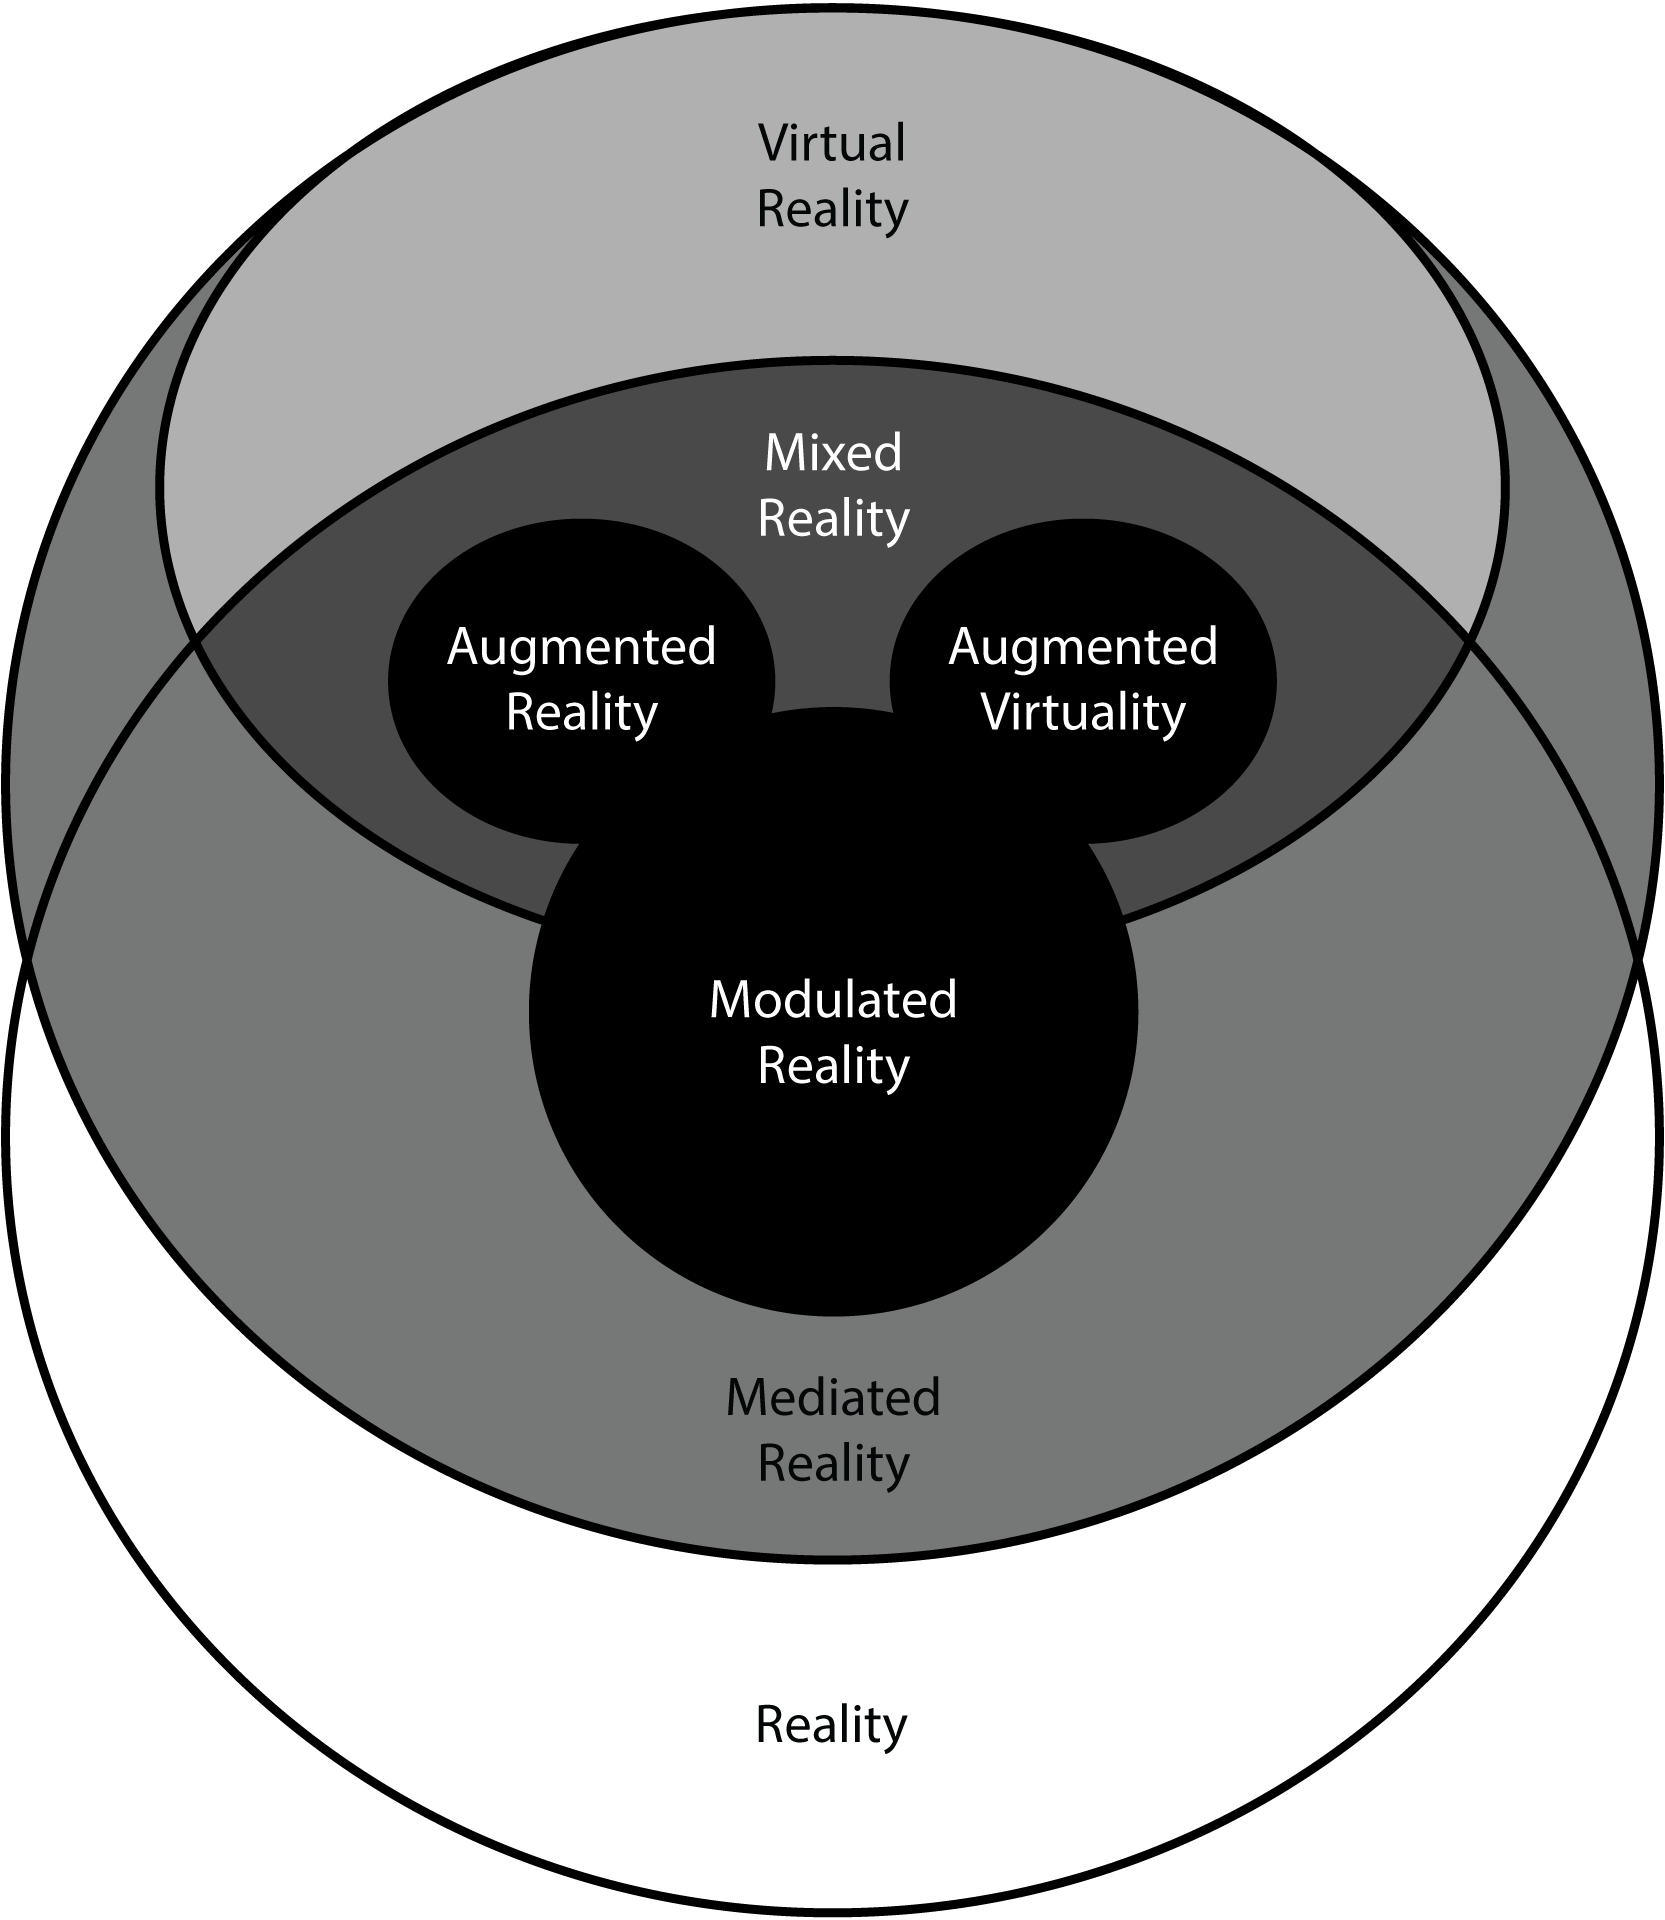
\includegraphics[width=0.5\linewidth]{Mann_venn_mod_3.png}
  \caption{Mann's Venn diagram of alternate realities after further modification.}
  \label{Mann_venn_mod_3.png}
\end{figure}

Visualising the position of the basic classes of reality and virtual reality using this same method requires more drastic alteration to the Venn diagram, but is diagnostic in further revealing the relationships between the terms covered in Mann's literature. The further modified Venn diagram (figure \ref{Mann_venn_mod_3.png}) shows that;
\begin{itemize}
	\item mixed reality is the intersection of reality and virtual reality;
	\item mediated reality can be comprised from purely real or purely virtual content;
	\item all virtual reality is necessarily mediated;
	\item modulated reality can comprise only mediated real, or both real and virtual aspects in a mixed reality;
	\item augmented reality and augmented virtuality can feature in modulated reality systems.
\end{itemize}

This final iteration of the Venn diagram still contains ambiguity, however it is more diagnostic for categorising the majority of alternate reality systems than the previous two diagrams, whilst also avoiding over-complication. There are two ambiguities to recognise. First, this diagram maintains from the original diagram positions in which a system can exist that is both mixed and modulated, but which is neither augmented reality nor augmented virtuality. Second, this diagram does not accommodate a purely virtual environment that is then modulated: whether such a system would ever be created is arguable though, as any modulation that could be performed by modulators external to the virtual environment software could almost certainly be better performed by the software itself.

%=========================================================================================================
%=========================================================================================================

%\clearpage

\section{Summary of Alternate Reality Definitions}
\label{summaryofalternaterealitydefinitions}
%Following are the definitions and identifying/classifying criteria for the different categories of alternate realities identified thus far in this chapter.

%This review has discovered differing (and in some cases conflicting) definitions for the different categories of alternate realities and for the criteria for differentiating between them. What follows in this section represents the definitions and differentiating criteria that this review has adopted after concluding them the most widely accepted and well reasoned.

%=========================================================================================================

\begin{center}
\begin{longtable}{ l p{10cm} }

\toprule

\textbf{Term} & \textbf{Definition} \\

\midrule

%=========================================================================================================
		
Reality & An environment that is entirely unmodelled, with the viewport containing no virtual objects and with no computer-based quantitative information associated with any of the (necessarily real) objects. \\
		
\midrule
		
%=========================================================================================================

Alternate Reality & Any environment in which the environmental stimuli received by a subject have been somehow mediated or modulated. That is, alternate reality is a term that encompasses everything that isn't purely `reality'. \\

\midrule
		
%=========================================================================================================

Telepresence & The ability for a user to experience a sense of presence at a real location remote to themselves~\cite{Sheridan1992a}. \\

%=========================================================================================================

Virtual Reality (VR) & The polar opposite of reality, an environment that consists solely of virtual objects, with computer-based quantitative information associated with and between all of them, creating a completely synthetic world entirely discrete and separate from the real world; a new world that exists solely within the data structures of a computer~\cite{Milgram1994, Milgram1999, Want2009}.

While traditional definitions of virtual reality require the environment to be completely immersive, such that when involved with the environment the user is completely unaware of the real environment that surrounds them (such as by using Head Mounted Displays and body tracking techniques to remove logical anchors to the real world~\cite{Druck2006}) the criteria adopted herein are less drastic, classifying the virtual environments presented by video games viewed via 2D monitors as rudimentary implementations of virtual reality; they are after all completely modelled environments that exist entirely separate to the real world. \\
		
\midrule
		
%=========================================================================================================

Distributed Virtual Reality (DVR) & Multi-user VR where telecommunications are employed to allow multiple (geographically distributed) users to occupy the same VR environment, allowing cooperation~\cite{Terashima2001}. \\

\midrule
		
%=========================================================================================================


Mixed Reality (MR) & The broad range of environments that arise from the merging of real and virtual environments to some extent, such that the result is neither entirely real nor entirely virtual, with real and virtual objects co-existing. Both augmented reality and augmented virtuality are included under the broader classification of mixed reality. \\

\hline
		
%=========================================================================================================

Augmented Reality (AR) & A mixed reality environment comprising a real environment that has had virtual objects added to or overlain upon it. A common approach for achieving this addition/overlay is superimposing virtual objects over a direct or indirect view of the real environment using Head Mounted Displays \&/or cameras~\cite{Krevelen2010}. \\

	%A commercial example of \textit{augmented reality} is the Layar browser for mobile phones, which overlays various forms of data onto the view captured by a phone's camera after determining its location and orientation using GPS, accelerometer and magnetometer readings~\cite{eishita:layar}

%~\cite{Milgram1999}

\midrule

%=========================================================================================================

Diminished Reality & Where augmented reality is concerned with adding virtual objects to a view of the real world, diminished reality is concerned with the removal or replacement of objects from a view of the real world~\cite{Mann2002}. Examples include the removal of real world advertisements (such as billboards). \\

\midrule

%=========================================================================================================

Augmented Virtuality (AV) & A virtual environment upon which sampled real objects are overlain, perhaps through the use of cameras~\cite{caballero:behand}. \\

%A simple commercial example of augmented virtuality is the EyeToy accessory and associated software for Sony's Playstation 2 games console (and later the Playstation Eye for the Playstation 3), a digital camera that captures images of players and their surroundings and integrates them into the gaming experience presented on the screen.

\midrule

%=========================================================================================================

Mediated Reality & \textit{``A general framework for artificial modification of human perception by way of devices for augmenting, deliberately diminishing, and more generally, for otherwise altering sensory input''}~\cite{Mann2002a}. Encompasses all of mixed reality and modulated reality. \\

\midrule

%=========================================================================================================

Modulated Reality & Platforms that aim to modify the user's view, by multiplicative, diminishing, rotational, etc. techniques, where the user's view can be wholly real, or a mix of real and virtual content. \\

\bottomrule
\caption{Summary of alternate reality definitions.}
\end{longtable}
\end{center}

%=========================================================================================================
%=========================================================================================================

\section{Additional Alternate Reality Terms}

In addition to the range of alternate realities covered in the previous section, there are several less commonly used terms that do not feature or fit well into the previously identified frameworks.

%=========================================================================================================

\subsection{HyperReality}
\label{subsec_HyperReality}

HyperReality (HR) is the term given to a hypothetical communications infrastructure that allows the seamless commingling of reality and virtual reality, human intelligence and artificial intelligence. In terms of the previously explored alternate reality terms, a HR system is most accurately described as facilitating the creation of mixed reality environments that bring virtual reality content into real world locations $-$ \textit{``It seeks to make virtual reality something that is experienced as part of physical reality, so that virtual and real phenomena appear to interact with each other: HR is VR as well as, not instead of, PR''}~\cite{Terashima2001}.

HR is an abstract, high level term that refers to a category of mixed reality environments that combine VR content with views of the real world in a manner that arguably falls under the moniker of augmented reality, however HR places emphasis on the integration of the virtual reality content into the real world in a seamless manner, such that HR enables hyperreality (this latter non-capitalised term referring to the postmodern usage of the word wherein an observer is unable to distinguish reality from a simulation of reality~\cite{Baudrillard1994}).

%``HyperReality (HR) is a hypothetical basic communications infrastructure that allows possible by information technology. It allows the commingling of physical reality with virtual reality and human intelligence with artificial intelligence.''

%``HyperReality (HR) is a technological capability, like nanotechnology, human cloning and artificial intelligence. Like them, it does not as yet exist in the sense of being clearly demonstrable and publicly available. Like them, it is maturing in laboratories where the question `if?' has been replaced by `when?' And like them, the implications of its appearance as a basic infrastructure technology are profound and merit careful consideration.''

%``The concept of HyperReality (HR), like the concepts of nanotechnology, cloning and artificial intelligence, is in principle very simple. It is nothing more than the technological capability to intermix virtual reality (VR) with physical reality (PR) and artificial intelligence (AI) with human intelligence (HI) in a way that appears seamless and allows interaction.''

%``The project that led to the concept of HR began with the idea of teleconferencing in virtual reality.

%ATR (Advanced Telecommunications Research) in Kansai Science City

%``HyperReality is a technological capability that makes possible the seamless integration of physical reality and virtual reality, human intelligence and artificial intelligence.''

%Must be seamless, without a `bezel' (HyperReality p142)

%``HR makes it possible for the physically real inhabitants of one place to purposively coact with the inhabitants of remote locations as well as with computer-generated imaginary or artificial life forms in a HyperWorld. ***PoSR link

%Distributed Virtual Reality - simply shared VR that is accessible by multiple simultaneous users via telecommunications infrastructure (HyperReality p13)

%HR is a single mixed reality environment (HyperReality p26)

%``It seeks to make virtual reality something that is experienced as part of physical reality, so that virtual and real phenomena appear to interact with each other: HR is VR \textit{as well as, not instead of,} PR.'' (HyperReality p31, emphasis original)

%HyperReality is a technological metaconcept (HyperReality p41)

%HyperReality is a technology that enables hyperreality (the postmodern term) (HyperReality p41)

%``HyperReality means a reality in which there is the extra dimension of virtual reality within normal physical reality'' (HyperReality p42)

%``The implication of HR is that, wherever you are, you could be somewhere else.'' (HyperReality p149) - not sure I agree with this as definition of HR though, as HR is about VR *as well as* rather than instead of PR - my mobile parallel reality is more like VR instead of PR, but with the ability of rapidly temporal change in which is being observed.

% =======

%From Simulacra and Simulation (Jean Baudrillard), Hyperreality is essentially an inability of consciousness to distinguish reality from a simulation of reality. Hyperreality is seen as a condition in which what is real and what is fiction are seamlessly blended together so that there is no clear distinction between where one ends and the other begins. It allows the commingling of physical reality with virtual reality (VR) and human intelligence with artificial intelligence (AI).

%=========================================================================================================

\subsection{PolySocial Reality}

PolySocial Reality (PoSR) describes situations in which people multiplex their physical reality, where they engage in face-to-face social interaction, with Web-based social networks and apps for Internet mediated social interaction. Instead of defining a new type of alternate reality in terms of the provenance of the audiovisual stimuli received by a subject, PoSR is more concerned with the provenance of the multiple, simultaneous social interactions that are mediated through various telecommunications media~\cite{Applin2012}. It has been shown that \textit{``effective interaction among participants is a contributing factor to presence''}~\cite{Terashima2001}, so it should not come as much surprise to observe people maintain PolySocial interactions between their real environment and a virtual one, as the opening quote to chapter \ref{introduction} from Waterworth and Waterworth posits will be the case.

%\textbf{*** Mention place vs non-place?}

%HyperReality p55, references Slate and Usoh 1994

%"Lifton does not fully address the social element and aspects of Dual Reality. In part, this results from the rather 'fixed' locations that he is linking, and by his restriction of the social components to those people in the lab who share both aspects of the dual reality. The introduction of mobility via phones and other devices to the context will require a generalisation of the concept of Dual Reality." Feb 2011

%"PoSR builds on a modification of Lifton's definition of Dual Reality: "An environment resulting from the interplay" among two or more dual realities." Feb 2011

%"At any given moment, as people are interacting with mobile devices in the 'non-place' they are intersecting and/or colliding with others in 'place', who may not own such devices." July 2011

%"...altering the physical space into a hybrid of concurrent 'place' and 'non-place'." July 2011

%"...within the context of the Future Internet, using terms like 'Augmented Reality', 'Dual Reality', 'Blended Reality', and 'Mixed Reality' ('Virtual Reality' is omitted for lacking interactivity with other worlds) may be limiting in scope. Those terms do not currently addres the multiplexing scenario that is commonplace amongst groups of people using the Internet simultaneously, each with a different multiplexed set of 'mixed' realities. The complete set of those multiplexed 'mixed realities' connected through the social networks that they reside within, we refer to by the name of PolySocial reality (PoSR)." July 2011

%"Lifton discusses the 'vacancy problem' in relation to users of virtual worlds both with respect to their (lack) of presence in their local 'reality' when engaged in a virtual world and the paucity of the virtual world when users are not engaged. He proposes that Dual Reality potentially address the 'vacancy problem' by making both the place (local reality) and the non-place (virtual reality) interoperable in some respects by mapping information from each to the other using real, or virtual, sensors. This is also a useful concept for discussing social and cultural issues arising from the increased use of technologies to support the user experience for augmented, mixed and blended realities. Lifton does not fully address the social element and aspects of Dual Reality. In part, this results from the rather 'fixed' locations that he is linking, and by his restriction of the social component to those people in the lab who share both aspects of the dual reality. The introduction of mobility via phones and other devices to the context will require a generalisation of Dual Reality. July 2011

%``Dual Realitiy relates to interoperability between the two realities through sensors and actuators, not simply by rendering one in the other.'' July 2011

%

%=========================================================================================================
%=========================================================================================================

\section{Cross Reality}
\label{sec_crossreality}

\newcommand{\SLfootnote}{\footnote{Second Life.}}

Cross reality (XR) is the ubiquitous mixed reality situation that arises from the fusion of real-world sensor/actuator infrastructure with virtual environments, such that augmented reality and augmented virtuality manifest simultaneously and facilitate synchronous bidirectional exchange of media and control information between real and virtual environments. Sensors collect and tunnel dense real-world data into virtual environments where they are interpreted and displayed to dispersed users, whilst interaction of virtual participants simultaneously incarnates into the real world through a plenitude of diverse displays and actuators~\cite{Paradiso2009}, such that actions within the virtual environment could have `extravirtual effects'~\cite{Soraker2010} upon the real environment and vice-versa (see also Brey~\cite{Brey2014} for further discussion about the ontology of real and virtual objects and actions).

The principle features that distinguish XR from the other alternate realities covered so far are;
\begin{enumerate}
	\item a shift from single- to bi-directional information flow between real and virtual environments~\cite{kim:practical};
	\item that both environments are complete unto themselves (but are enriched by their ability to mutually reflect, influence and merge into one another).~\cite{lifton:merging}
\end{enumerate}

%This thesis presents systems that focus on the second aspect above and extends it by permitting both environments to be experienced at any time and position.

XR as an alternate reality paradigm has its roots in work undertaken by the IBM Virtual Universe Community~\cite{Hughes2006, Hughes2006a,Hughes2006b}, described in personal correspondence by Ian Hughes;

\begin{quote}
\textit{``The control mechanisms worked two ways generally. There was a physical lab that had devices that were controlled by a pub/sub mechanism \ldots\ Those devices subscribed to various messages. So initially web pages controlled them \ldots\ Equally the objects generated messages when they were physically switched on and off. As SL\SLfootnote{} had an RPC interface it was possible \ldots\ to subscribe to the same messages and send requests into SL to change states of object \ldots\ So there were lights, blinds, proximity detectors and even the tilt sensors on the laptops that were instrumented with these messages.''}
\end{quote}

It was the work of the Responsive Environments Group at MIT's Media Lab, centred around the research of Joshua Lifton in combining the Plug sensor/actuator platform~\cite{Lifton2007b} with a Second Life hosted virtual model of the physical Lab (\ref{lifton_shadow_lab.png}) in the `Shadow Lab' project, that truly launched XR as a research area. The Shadow Lab project did not allow for tandem visual engagement with both constituent environments of the cross reality platform, focussing instead on the interplay of sensor data and actuator commands exchanged between the environments. The visual aspect was addressed in part by the subsequent Ubiquitous Sensor Portal project, which situated 45 I/O rich `portals' (figure \ref{ubiquitous_sensor_portal.jpg}) throughout the Lab, each with a corresponding extension in Second Life. However in stark contrast to the earlier Shadow Lab project, the virtual portals were not situated in a simulation of the real Media Lab in situations corresponding to their physical location, but instead used a more abstract virtual representation with a geometric layout reflecting intellectual affiliation as opposed to real-world location.

\TwoFig{lifton_shadow_lab.png} {Side view of the virtual Shadow Lab.} {lifton_shadow_lab.png}
       {ubiquitous_sensor_portal.jpg} {A Ubiquitous Sensor Portal.} {ubiquitous_sensor_portal.jpg}

One of the driving motivations behind this work was what Lifton dubbed `the vacancy problem';

\begin{quote}
\textit{``the noticeable and profound absence of a person from one world, either real or virtual, while they are participating in the other. Simply put, the vacancy problem arises because people do not currently have the means to be in more than one place (reality) at a time.''}~\cite{Lifton2007a}
\end{quote}

Which the Shadow Lab addressed via the sensor/actuator infrastructure to more closely link the real and virtual environments, such that actions and events in one could manifest and be observed by users in the other even if they could not directly visually observe both environments in tandem. The vacancy problem was previously observed by HR researchers, touching on an observation of the PoSR situations observed among mobile phone users of the time as a manifestation of the problem before virtual environments were introduced to the picture; %HyperReality p35

\begin{quote}
	\textit{``One of the main problems with \ldots\ virtual reality is what to do about the body that is left behind in physical reality \ldots\ In HyperReality a person by definition is perceptually aware of the physical world around them, yet part of the attention normally given to the physical reality is given to interacting with virtual reality. It is difficult as yet to see how much this matters, but the increasing use of the mobile phone, which is a primitive form of HR, gives us some feel for the issues. People using a mobile phone can walk busy streets \ldots\ while talking to someone who is not there.''}~\cite{Terashima2001}
\end{quote}

\textbf{***Briefly mention standards, mainly ISO/IEC 23005 (MPEG-V)}

%=========================================================================================================

\subsection{Alternate Reality Definitions from Cross Reality}

Lifton's use of alternate reality terminology does not directly conclude that MR is a broad term encompassing both AR and AV, but defines it as an environment ;

\begin{quote}
	\textit{``\ldots\ which would be incomplete without both its real and virtual components. For example, the walls and windows of a mixed reality house might be real, but the view out the windows might be virtual, either generated by a projector or as a blue screen effect in a head-mounted display. Without both the real house and the virtual views out the windows, the illusion of a consistent reality is broken''}~\cite{Lifton2007a}
\end{quote}

The diagram Lifton presents (figure \ref{original_lifton_axis.png}) alludes to Milgram's continua but places MR, under the above definition, as a separate classification of alternate reality between AR and VR. Lifton does not mention AV, even though the XR systems he presents arguably cause it to manifest. Figure \ref{modified_lifton_axis.png} is the result of modifying this diagram to match the definitions adopted by this chapter in section \ref{summaryofalternaterealitydefinitions}.

\begin{figure}[h]
	\centering
	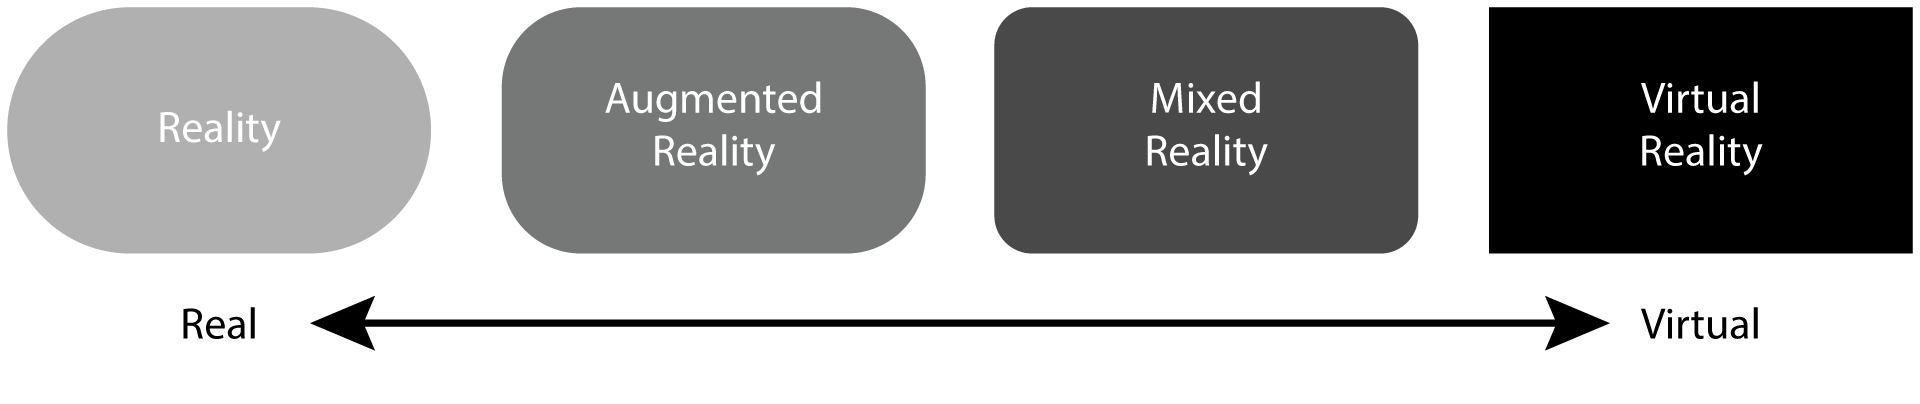
\includegraphics[width=.8\textwidth]{Lifton_continuum_original.png}
	\caption{Lifton's virtual worlds taxonomy.}
	\label{original_lifton_axis.png}
\end{figure}

\begin{figure}[h]
	\centering
	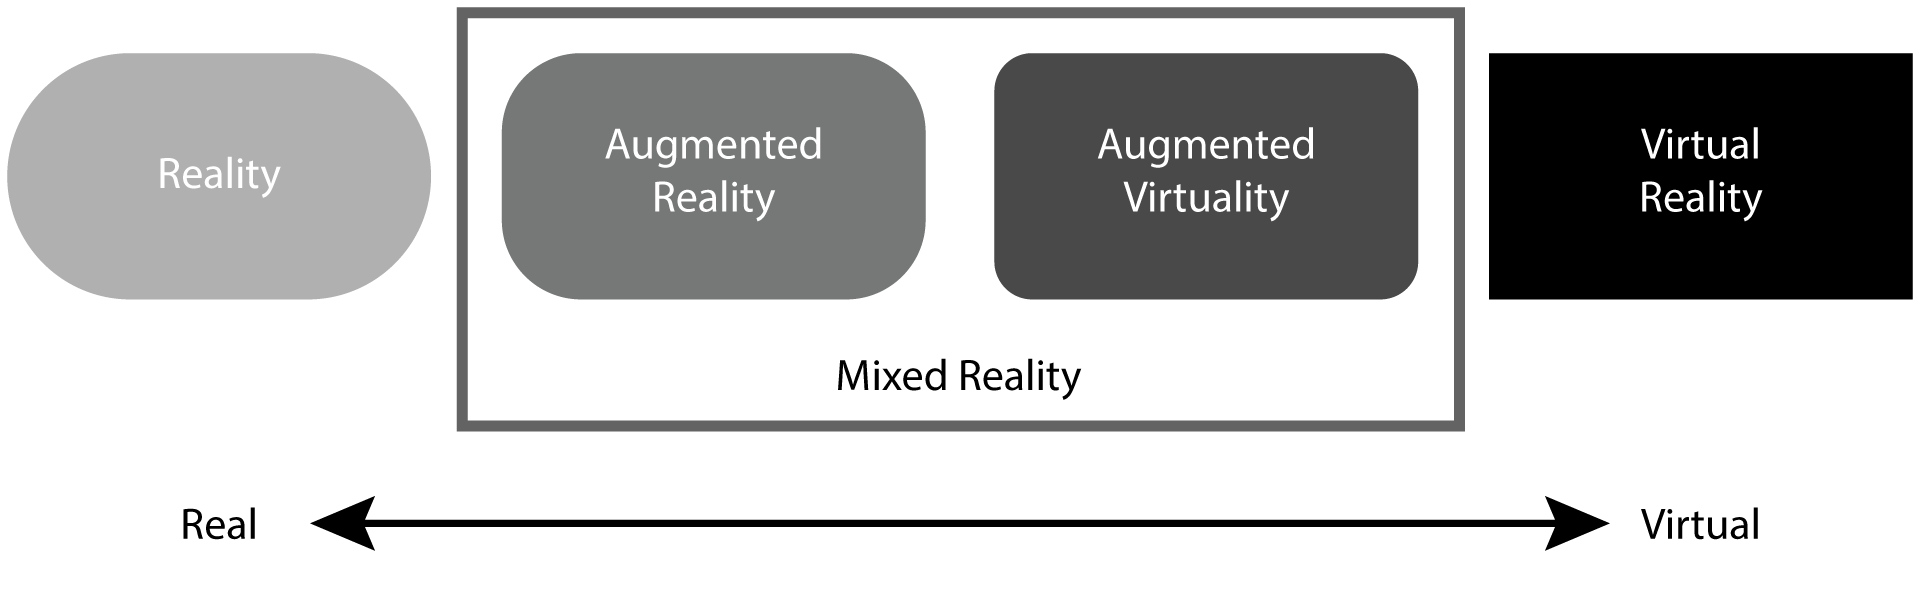
\includegraphics[width=.8\textwidth]{Lifton_continuum_modified.png}
	\caption{Lifton's virtual worlds taxonomy after modification.}
	\label{modified_lifton_axis.png}
\end{figure}

Lifton does however explain that while such a taxonomy can be successfully applied to most alternate realities, with each falling into a different singular category, it does not well address those that feature two complete realities, one real and one virtual, which is one of the defining and distinguishing characteristics of a XR system and instead prefers figure \ref{reality_virtual_reality_sensor_networks.png} to show how sensor/actuator infrastructure can cause the real and a virtual environment to merge into a cross reality.

\begin{figure}[h]
	\centering
	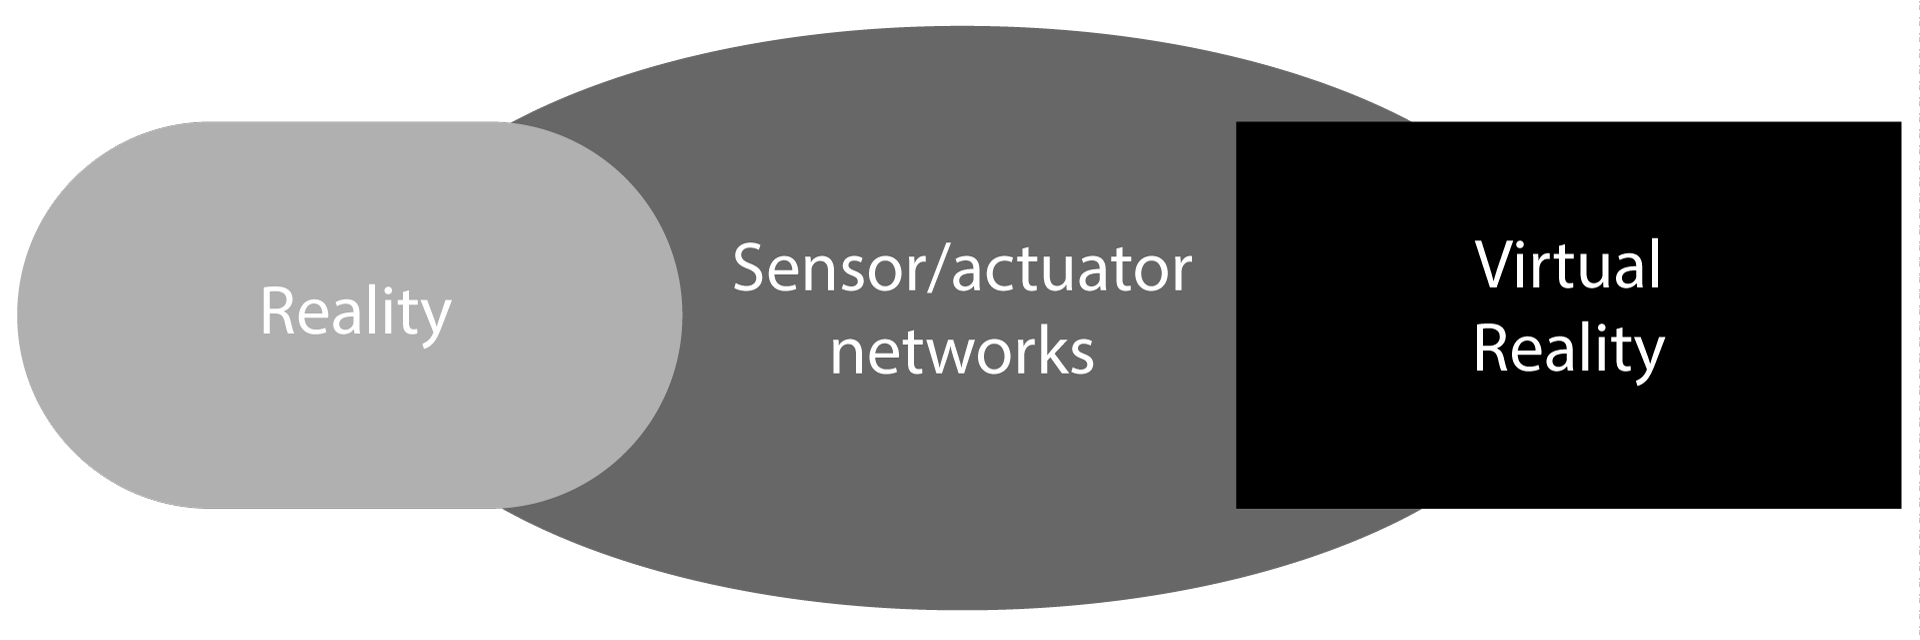
\includegraphics[width=.6\textwidth]{reality_virtual_reality_sensor_networks.png}
	\caption{Sensor/actuator infrastructure merging real and virtual environments into an instance of XR.}
	\label{reality_virtual_reality_sensor_networks.png}
\end{figure}

%page 37 of Lifton's thesis

%=========================================================================================================

\subsection{Position of Cross Reality}

\label{positionofcrossreality}

\newcommand{\avxrfootnote}{\footnote{This discussion over the relationship between AR and XR also stands for the relationship between AV and XR, however as AV has received less attention in the literature and in commercially available implementations, the discussion uses AR as its example.}}

The position of XR in relation to other alternate realities can be visualised using Milgram and Kishino's virtuality continuum. As one of the defining characteristics of a XR system is that it features two environments, both complete unto themselves, the explanation herein distinguishes between environments themselves (depicted in figures \ref{virtuality-continuum-augmented-reality} to \ref{virtuality-continuum-cross-reality-information-flows-dashed.png} by solid ellipses) and where the stimuli that the user is perceiving originate from (depicted by dashed ellipses).

%Ontology - The core meaning within computer science is a model for describing the world that consists of a set of types, properties, and relationship types. There is also generally an expectation that the features of the model in an ontology should closely resemble the real world (related to the object).

Of particular importance is to appreciate the distinction between a XR system and an AR system\avxrfootnote{}, as both concepts involve user engagement with both real and virtual content. Whilst an AR system features a single environment, comprised of the user's RW overlain by some virtual content, with the user perceiving stimuli from this single augmented environment (figure \ref{virtuality-continuum-augmented-reality}), a XR system instead features two discrete environments, one real and the other virtual, each complete unto itself (figure \ref{virtuality-continuum-cross-reality-1}), with the user attending either to the stimuli originating from the real environment (figure \ref{virtuality-continuum-cross-reality-2}) or to the stimuli originating from the virtual environment (figure \ref{virtuality-continuum-cross-reality-3}). Similarly to AR, a HR environment likewise constitutes a single physical environment, formed by the seamless introduction of VR content into the real world, rather than two complete environments;

%`physical' quote is HyperReality p158

%HyperReality p26
\begin{quote}
	\textit{``\ldots\ virtual people, virtual objects and virtual settings can interact and thereby communicate with real people, real objects and real settings as though they were all part of the same world.''}~\cite{Terashima2001}
\end{quote}

Although a XR system as a whole should definitely be considered a case of MR, whether each of its constituent environments should be considered outwith or within the realm of MR (especially when visualised upon the continuum) is open to debate. Taking the real environment as an example, one could argue that the use of actuators to produce physically observable effects on behalf of controls from the virtual environment constitutes an AR environment. However in adhering to the definition of AR adopted earlier (see section \ref{summaryofalternaterealitydefinitions}) we would not label this an AR environment as we do not have \textit{virtual} objects overlain upon our view of the real environment, but rather \textit{real} objects controlled by the actions and events of a discrete virtual environment. So whilst an AR environment falls within the realms of MR, the constituent environments of a XR system when considered individually are considered as occupying the two extremes of the continuum, outwith the MR region and thus their depiction as such in figures \ref{virtuality-continuum-cross-reality-2} and \ref{virtuality-continuum-cross-reality-2}. It is beyond the scope of this thesis to discuss the ontological implications of the `reality' of virtual objects and actions, so the reader is referred to Brey~\cite{Brey2014} for further discussion of this subject.

%***this is more to do distribution of the dashed line surrounding the environments, rather than the position of the environments themselves (solid line)***

%However, XR systems that allow simultaneous interaction with both of their constituent environments blur this definition; using a XR platform such as that discussed in this document, a user can transition between perceiving stimuli from each of these environments (figures \ref{virtuality-continuum-cross-reality-2} and \ref{virtuality-continuum-cross-reality-3}) in a manner that allows them to engage with each environment without becoming wholly vacant from the other.

A further distinction between AR and XR is made by considering Steed's primary environment concept. For an AR system the primary environment is necessarily real, as AR describes systems in which virtual objects are superimposed upon a view (a background) of a real environment. However for an XR system one could argue that the primary environment is either real or virtual, depending upon how the user interacts with the system. For the user that walks through the RW environment of an XR system and views their unmediated surroundings (including actuations trigger by events within the VR environment), one would intuitively posit that their primary environment is real. But for the user that sits in front of a computer monitor and uses an avatar to walk through the VR environment of the same XR system and views the avatar's VR surroundings (including visualisations of sensor data collected from the RW environment), one would posit that their primary environment is virtual. Considering figures \ref{virtuality-continuum-cross-reality-2} and \ref{virtuality-continuum-cross-reality-3} again, one could say that the dashed ellipses thus represent the primary environment.

\begin{figure}[h]
	\begin{center}
		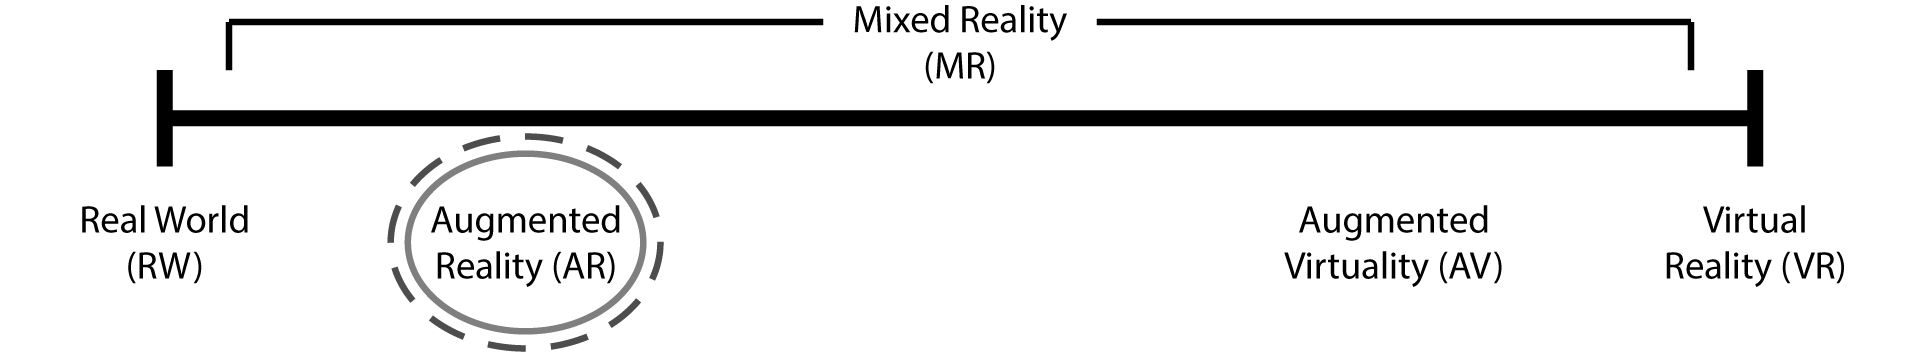
\includegraphics[width=\textwidth]{virtuality-continuum-augmented-reality.png}
		\caption{AR visualised using Milgram \& Kishino's reality-virtuality continuum.}
		\label{virtuality-continuum-augmented-reality}
	\end{center}
\end{figure}

\begin{figure}[h]
	\begin{center}
		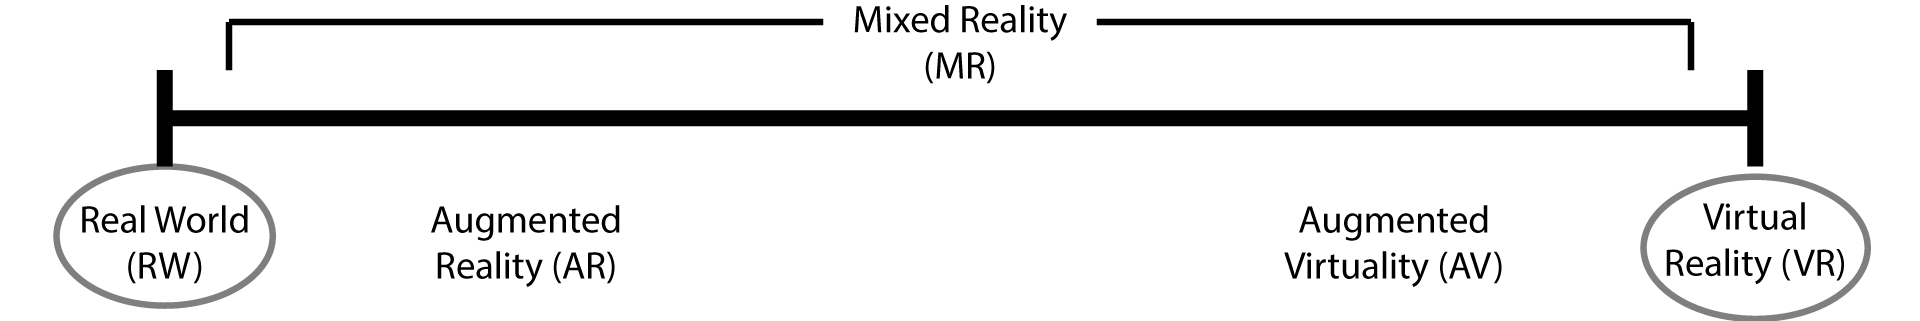
\includegraphics[width=\textwidth]{virtuality-continuum-cross-reality-1.png}
		\caption{The two environments that comprise a XR system visualised using Milgram \& Kishino's reality-virtuality continuum.}
		\label{virtuality-continuum-cross-reality-1}
	\end{center}
\end{figure}

\begin{figure}[h]
	\begin{center}
		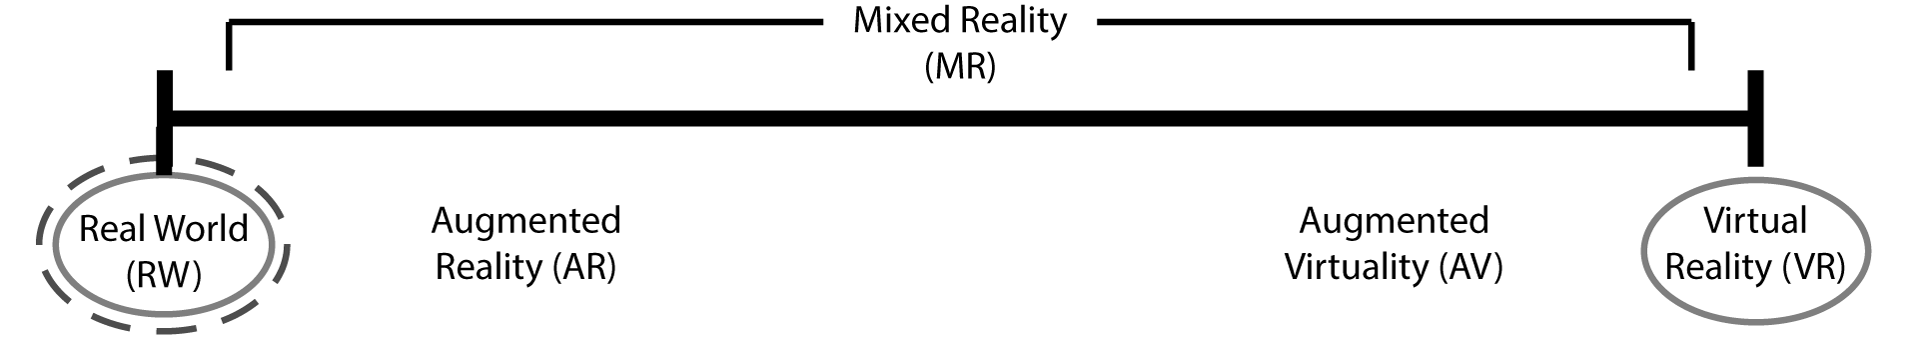
\includegraphics[width=\textwidth]{virtuality-continuum-cross-reality-2.png}
		\caption{A XR system with the user attending to RW stimuli, visualised using Milgram \& Kishino's reality-virtuality continuum.}
		\label{virtuality-continuum-cross-reality-2}
	\end{center}
\end{figure}

\begin{figure}[h]
	\begin{center}
		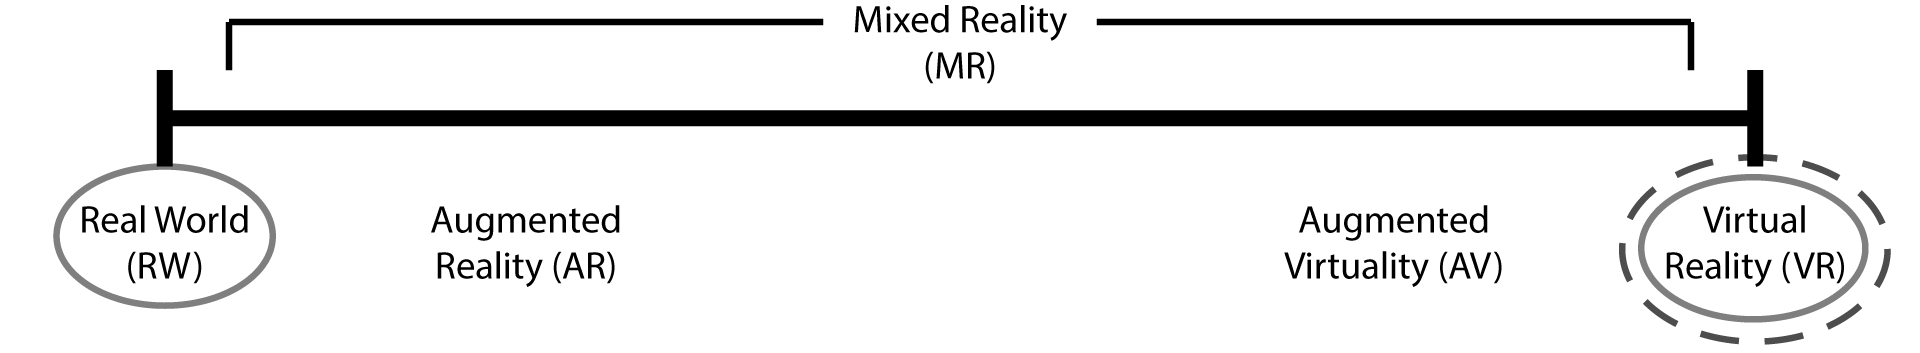
\includegraphics[width=\textwidth]{virtuality-continuum-cross-reality-3.png}
		\caption{A XR system with the user attending to VR stimuli, visualised using Milgram \& Kishino's reality-virtuality continuum.}
		\label{virtuality-continuum-cross-reality-3}
	\end{center}
\end{figure}

%=========================================================================================================

\section{Parallel Reality}

\newcommand{\PRfootnote}{\footnote{Note that the use of `PR' in the quotation in section \ref{subsec_HyperReality} is a reference to `physical reality' (that author's term for what this thesis simply calls `reality') and is not a reference to parallel reality.}}

The discussion in the previous section highlighted that the first distinguishing factor of XR, that differentiates it from other alternate realities such as AR and AV, is that XR features two discrete environments, one real and one virtual. The second distinguishing factor is the presence of a bidirectional flow of information between these two environments (figure \ref{virtuality-continuum-cross-reality-information-flows-dashed.png}, an integration of figure \ref{reality_virtual_reality_sensor_networks.png} with Milgram and Kishino's virtuality continuum).

\begin{figure}[h]
	\begin{center}
		
\includegraphics[width=\textwidth]{virtuality-continuum-cross-reality-information-flows-dashed.png}
		\caption{The two environments that comprise a XR system, plus the bidirectional information flow between them, visualised using Milgram \& Kishino's reality-virtuality continuum.}
		\label{virtuality-continuum-cross-reality-information-flows-dashed.png}
	\end{center}
\end{figure}

While the concept introduced by this thesis features two discrete environments, one real and one virtual, that users can transition between visually observing (figures \ref{virtuality-continuum-cross-reality-2} and \ref{virtuality-continuum-cross-reality-3}), it does not feature this bidirectional information flow between the environments (other than using sensed real position information to maintain the user's vantage point into the virtual environment). Thus, this concept cannot be considered a XR system as it does not meet both of the distinguishing criteria. The term \textbf{parallel reality} (PR\PRfootnote{}) is instead proposed to describe this concept. Parallel reality is thus defined as;

\begin{quote}
	\textbf{Parallel Reality (PR):} A system comprising two environments, one real and the other virtual, each complete unto itself and wherein the user may freely switch between them.
\end{quote}

Should a bidirectional information flow be introduced to a PR system, or the ability to transition between receiving stimuli from either environment be introduced into a cross reality system, one would effect \textit{parallel cross reality}.

Picking up the discussion of primary environments once more, if one follows the reasoning that the primary environment of an XR system depends upon the method with which the user interacts with the system, it stands that a PR system is one that provides the user the ability to change this method and thus change their primary environment. In this regard we further distinguish a PR system from an AR system, by defining it as one that allows its users to switch between two different primary environments rather than one that augments one particular primary environment.

%=========================================================================================================

\subsection{Spatial Equivalence in Parallel Reality}

\label{spatial-equivalence}

%(Life on the Screen, p219
\newcommand{\turklevrfootnote}{\footnote{\textit{``For virtual reality to be interesting it has to emulate the real. But you have to be able to do something in the virtual that you couldn't in the real.''}~\cite{Turkle1997}}}

When discussing a PR system that allows a user to transition between two environments, one real and the other virtual, one must consider the relationship between the two environments, namely whether (\& if so, to what extent) their layout, dimensions and content relate to each other, a consideration we will refer to as their \textit{spatial equivalence}.

This distinction depends partly upon whether one adopts a dualistic concept of virtual space experience, wherein `cyberspace' is a space in its own right with its own logic and metaphysics thus capable of playing host to any number of fantastical things and places, or whether one restricts the virtual environment by following a positivistic understanding of virtual space in which it serves only as a representation of real - using cyberspace for \textit{``creating acceptable substitutes for real \ldots\ environments''} instead of for \textit{``constructing imaginary worlds that are indistinguishable from the real world''}~\cite{Qvortrup2002}. One may also wish to consider this distinction in relation to the different stages identified by Baudrillard between simulacra and simulation, with complete spatial equivalence occupying the first stage of a faithful image or copy of a profound reality (the positivistic position), zero spatial equivalence occupying the fourth stage of pure simulation with no relation to anything in reality (the dualistic position) and partial equivalence perhaps occupying the second stage, a perversion of reality~\cite{Baudrillard1994}.

%=========================================================================================================

However one treats virtual space, a PR system would be unrewarding if the real and virtual environments were identical\turklevrfootnote{}. However a virtual environment that shares roughly the same fundamental dimensions and layout as the real environment (representing the same `place') but presents an \textit{alternative} representation of it has been proven to be a useful modality in previous XR research (see section \ref{sec_crossreality}) and it is this arrangement that this thesis explores, in particular where the virtual environment represents the same place as the real environment but at an earlier moment in time.

One might consider the `Second Earth' concept to be the ultimate realisation of this scenario of spatially equivalent real and virtual environments. The combination of virtual world technology (as in Second Life) with `mirror world' technology (as in Google Earth), Second Earth theorises a virtual simulation/reconstruction of the entire physical world, such that for any location in the real world there is a corresponding location in the virtual world~\cite{Roush2007}. The PR platforms developed in this thesis focus on individual locations, however it does not take a great leap of the imagination to comprehend the worth of such a system scaled to a larger, even global, size.

Although the use cases for PR systems that feature completely unrelated real and virtual environments (including where the virtual environment is entirely fictitious) may seem limited in terms of possible benefits to understanding or knowledge gain when comparing and contrasting the environments, an educated approach to implementing transitions between these environments, that takes similar considerations as the platforms developed in this thesis, does conceivably have purpose. In the opening quote to this chapter, taken from Neal Stephenson's cyberpunk novel \textit{Snow Crash}, the protagonist enquires about the location of another character, called Y.T., both in the real world and in the `Metaverse'. For the sake of this discussion, the Metaverse can be considered analogous to a virtual world akin to Second Life, accessed via a head mounted display, and comprises an entirely synthetic virtual world whose locations have no counterparts in the real world. Y.T.'s response is that \textit{``In  the Metaverse, I'm on a plusbound monorail train. Just passed by Port 35.''} whilst in reality she is at a \textit{``Public terminal across the street from a Reverend Wayne's"}.

In this scenario there is no spatial equivalence between the real environment and the virtual environment - they are not the same `place', however the protagonist still wishes to be able to experience both by transitioning between them, paying attention to one while travelling through the other. While this situation is currently science fiction, recent developments in mobile VR platforms such as Samsumg Gear VR\footnote{\url{http://www.samsung.com/global/microsite/gearvr/}} hint that we are not so far away from a time in which members of the general public will wish to multiplex their real environment with a virtual one while in public, in the same way that people commonly engage in computer-mediated communication (CMC) via their smartphones at the same time as walking through real environments and conversing with the people in them, creating instances of PoSR. If a PR system were to allow interaction between its user and other virtual environment users who are not part of the PR scenario, it is conceivable that PolySocial instances would arise, with PR users socially engaging both with people in their immediate RW environment and with people in their immediate VR environment, even where the latter are not present in the RW environment. This situation would present \textit{``\ldots\ instances of synchronous PoSR, multiple presence \ldots\ being activated in different environments.''}\footnote{Personal correspondence with Sally Applin, PoSR author.}

With the majority of players of popular Massively Multiplayer Online games (MMOs) wishing they could spend more time playing, over a fifth even wanting to spend all of their time in game~\cite{Castronova2006}, and with social roles and the community aspect constituting key aspects of these game's popularity~\cite{Castronova2006, Bartle2004}, informing the implementation of transitions between real and virtual in such systems with the findings of the experiments in this thesis into spatially equivalent PR systems promises to be beneficial to the further development of 3D social CMC.

%=========================================================================================================

\section{Summary of Additional Alternate Reality Definitions}
\label{summaryofadditionalalternaterealitydefinitions}

\begin{table}[h]
\begin{center}
\begin{tabularx}{\textwidth}{l *{2}{>{\centering\arraybackslash}X}}

\toprule

\textbf{Term} & \textbf{Definition} \\

\midrule

%=========================================================================================================
		
HyperReality (HR) & A hypothetical high level term referring to a category of mixed realities that combine VR content with views of the real world in a seamless manner such that the observer experiences \textit{hyperreality}. \\
		
%\hline
\midrule
		
%=========================================================================================================

hyperreality & A postmodern term describing a situation wherein an observer is unable to distinguish between reality and a simulation of reality. \\

%\hline
\midrule

%=========================================================================================================
		
PolySocial Reality (PoSR) & Describes multiple simultaneous social interactions mediated via various CMC technologies.~\cite{Applin2012}. \\

%\hline
\midrule

%=========================================================================================================

Cross Reality (XR) & Systems that feature two environments, one real and one virtual, both complete unto themselves~\cite{lifton:merging} but enriched by their ability to mutually reflect, influence and merge into one another thanks to bidirectional information flow between them~\cite{kim:practical}. \\

%\hline
\midrule

%=========================================================================================================

Parallel Reality (PR) & Systems comprising two environments, one real and the other virtual, each complete unto itself and wherein the user may freely switch between them. \\

%\hline

%=========================================================================================================
\bottomrule
\end{tabularx}
%\end{longtable}
\end{center}
\caption{Summary of additional alternate reality definitions.}
\end{table}

%=========================================================================================================
%=========================================================================================================

%\pagebreak
%next section was rendering off the page

\section{Presence}
\label{lit-review-presencec}
Any investigation into alternate realities, virtual reality in particular, is likely to involve discussion of \textit{presence} - the subjective experience of `being in' one place or environment, even when one is physically situated in another~\cite{Witmer1998}. Presence is distinguished from the concept of \textit{immersion}, an objective description of a technology describing the extent to which it is capable of delivering an illusion of reality to the senses of the user~\cite{Slater1997}. In current theoretical models, the sense of presence is seen as the outcome, or a direct function of, immersion; the more inclusive, extensive, surrounding and vivd the virtual environment is, or the more similar the transformations in the virtual environment are to those in the real world, the higher the sense of presence~\cite{Constantin2003}.

Related is the concept of \textit{involvement}, defined in this context as the psychological state experienced as a consequence of focusing one's energy and attention on a coherent set of stimuli and it is theorized that both involvement and immersion are necessary for experiencing a sense of presence~\cite{Witmer1998}.

\subsection{Waterworth and Waterworth's three dimensions of virtual experience}
\label{waterworthandwaterworth}
\newcommand{\presencefootnote}{\footnote{\textbf{Presence} in the context of this model is defined as a state of heightened perceptual processing of environmental stimuli (\textit{``a psychological focus on direct perceptual processing''}~\cite{Waterworth2001}) accompanied by lessened conceptual reasoning, whether these environmental stimuli originate from a real environment, a virtual environment, a mixed reality environment, or even from multiple discrete environments.}}

\newcommand{\absencefootnote}{\footnote{\textbf{Absence} is defined as \textit{``a psychological focus on \ldots\ conceptual processing''}~\cite{Waterworth2001}.}}

This notion of the sense of presence depending upon multiple factors is explored further by Waterworth and Waterworth who present the \textit{three dimensions of virtual experience} model~\cite{Waterworth2001}. In this model, the \textit{locus of attention} axis represents the environment where the stimuli that the user is perceiving originate from; the \textit{focus of attention} axis represents the balance between conceptual/abstract reasoning and perceptual/concrete processing, where complex conceptual reasoning results in little attention being paid to processing environmental percepts (whether originating from real stimuli, virtual stimuli, or a mix) thus reducing presence\presencefootnote{} in that environment toward its antithesis $-$ absence\absencefootnote{}; and the \textit{sensus of attention} axis represents the level of conscious arousal (or `wakefulness'~\cite{Laureys2009}) of the user, whether directed toward percepts originating from real stimuli, virtual stimuli, a mix of both, or not directed toward any percepts in the case of completely `absent' conceptual reasoning, a concept that is clarified by the authors in a subsequent publication;

\begin{quote}
	\textit{``Presence arises from active awareness of our embodiment in a present world around us. Presence is not consciousness, and we may be highly conscious while feeling absent, at those times when we are relatively unaware of our own embodiment.''}~\cite{Waterworth2014}
\end{quote}

In this model, the notion of \textit{involvement} relates closely to the \textit{focus of attention} axis; heightened involvement pertains to concentrating on environmental stimuli or meaningfully related activities and events, while heightened focus pertains to increased perceptual/concrete processing; lessened involvement pertains to a preoccupation with personal problems or activities occurring outwith the environment of interest, while lessened focus pertains to increased conceptual/abstract reasoning.

Similarly, a relationship can be drawn between the Waterworth model and Milgram and Kishino's reality-virtuality continuum, with the latter considered here to be analogous to the \textit{locus of attention} axis. The combination of these two models in this manner gives rise to the combined Milgram/Waterworth model which is shown by figure \ref{focus-locus-sensus-with-virtuality-continuum} and allows for a novel method of visualising the experience of using alternate reality systems, including parallel reality ones.

\begin{figure}[h]
	\begin{center}
		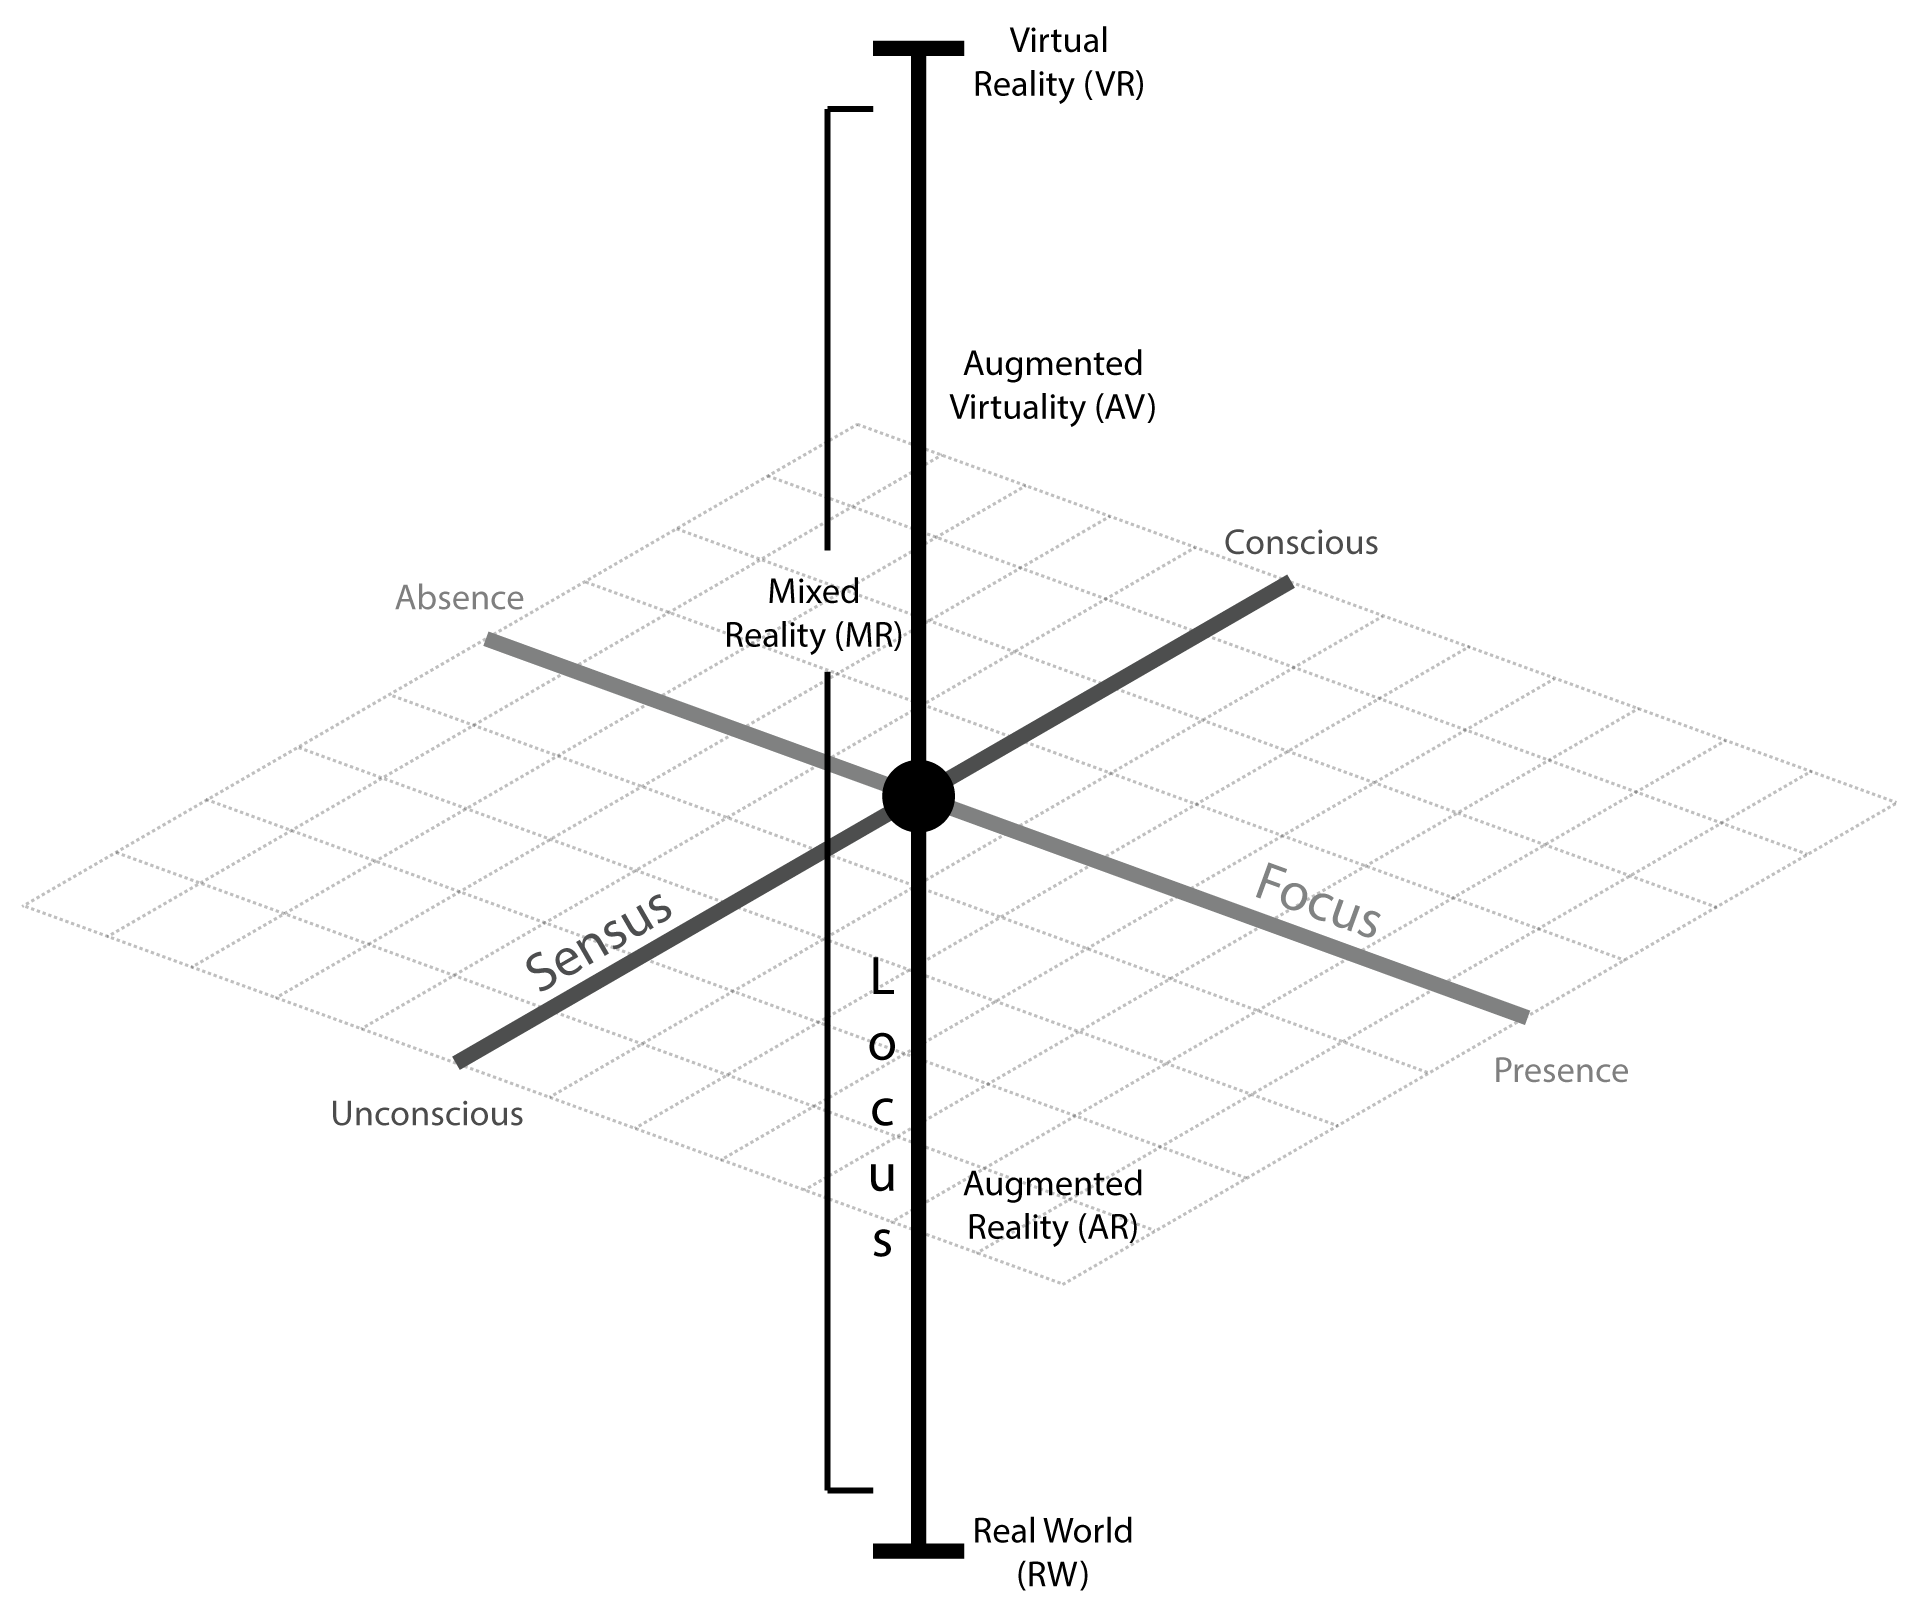
\includegraphics[width=.8\textwidth]{focus-locus-sensus-with-virtuality-continuum-updated-with-grid.png}
		\caption{The combined Milgram/Waterworth model.}
		\label{focus-locus-sensus-with-virtuality-continuum}
	\end{center}	
\end{figure}

Regarding the combined Milgram/Waterworth model shows more clearly that the balance between presence and absence relates to any environment upon the locus of attention axis, as confirmed by Waterworth and Waterworth in a subsequent publication;

\begin{quote}
	\textit{``We may feel hardly present at all in the physical world (a state we call absence) if nothing is happening there that is of interest or that impacts on our well-being, and so it is with mediated presence.''}~\cite{Waterworth2014}
\end{quote}

Furthermore one can postulate as to the essence of Lifton's vacancy with regard to the combined Milgram/Waterworth model (and thus to the experience of presence in general). Lifton's original definition presents vacancy as the `absence' of a person from one world while they are participating in the other, however the use of this term in Lifton's context differs to its use in the combined Milgram/Waterworth model. Lifton's absence refers to the inability to simultaneously perceive environmental stimuli from \textit{``more than one place (reality)''} while the absence of the combined Milgram/Waterworth model refers to increased conceptual/abstract reasoning resulting in a reduction of perceptual/concrete processing of environmental stimuli. In terms of the combined Milgram/Waterworth model, the vacancy problem should be thought of as referring to the largely singular nature of a user's position upon the locus of attention axis and the ability of a parallel reality platform toward reducing the problem, by allowing a user to `participate' in two environments at once, can be visualised either as extending the occupiable position upon the locus of attention axis from a singular position to a pair of positions (or as a range between two positions), or as reducing the deflection experienced upon the focus of attention axis from presence toward absence when performing a transition between two positions upon the locus of attention axis.

%The Sensus Dimension - the importance of being awake in class
%"Even as we sleep dreamlessly..." (example of being 'unconscious' in this regard)

%fourth axis is alterity, between hermeneutics and embodiment

%=========================================================================================================
%=========================================================================================================

\section{Transitions in Parallel Reality}

\label{transitions_in_parallel_reality}

\newcommand{\breakinpresencefootnote}{\footnote{The definition of \textbf{break in presence} adopted herein is the second from Waterworth and Waterworth~\cite{Waterworth2001} (p205): a movement along the focus axis away from presence in the real or a virtual environment and toward absence, which also relates to a reduction in involvement. This differs to Slater and Steed's original definition in~\cite{Slater2000} as they considered presence only in terms of attending to stimuli from a virtual environment, with a break in presence as a Gestalt switch to instead attending to stimuli from the real environment. Waterworth and Waterworth's model considers presence in terms of attending to stimuli from either the real \textit{or a virtual} environment, with a break in presence representing absence in the sense of heightened conceptual load and the resultant reduced perceptual processing of environmental stimuli originating from \textit{either} the real or a virtual environment. This definition better fits the situation invoked by the system developed in this thesis, which is concerned with intentionally and willingly switching engagement between stimuli from both real and virtual environments, rather than engaging with stimuli from only a virtual environment in a scenario where stimuli from the real environment are considered a `distraction'.}}

The novel aspect of PR is the ability it imparts upon its user to switch their locus of attention between equivalent vantage points in RW and VR environments. In order to achieve the highest quality of experience with this style of interaction with a PR system, it is vital to determine how best to implement the transitions; that is, to mitigate the increased cognitive load (manifesting as increased conceptual reasoning and reduced perceptual processing) required to comprehend each transition, as increased cognitive load will detract from engagement with the environments and reduce the user's willingness to perform subsequent transitions.

%In the systems developed by this thesis the users maintain mobility, such that they can move around the two environments in tandem, thus extending existing XR platforms that featured static locations at which a user in the real environment could see into the virtual and vice-versa. This combination of unhindered mobility with the ability to transition between real and virtual stimuli thus alleviates the vacancy problem.

%This is achieved by the user performing transitions between RW visual stimuli and VR visual stimuli, both presented via their HMD. This extends existing XR research by allowing the user to engage with the visual stimuli of the VR component of a XR system from any position and at any time.

Whilst some researchers support the notion that in systems where more than one environment competes for the user's locus of attention there is an `all or nothing' Gestalt switch between awareness of one environment and the other~\cite{Slater2002}, which would result in a substantial increase in cognitive load upon each transition, the position adopted by this thesis is of the contrary opinion; that switching locus of attention from the stimuli of one environment to those of another does not completely overrule the user's awareness of the former, that both environments can be perceived at the same time (albeit one to a lesser extent)~\cite{Ijsselsteijn2001} and that when engaging with VR content a user's focus can even be said to typically be \textit{shared} between VR and RW~\cite{Waterworth2001}, leading to a notion of `distributed' presence, or simultaneously experiencing a sense of presence in multiple environments.

This latter position is particularly apt for situations wherein the RW and VR environments share the same fundamental layout and dimensions (spatial equivalence), as those of the PR systems explored within this thesis do, as inherent familiarity between two environments intuitively reduces the cognitive load associated with transitioning between them.

Furthermore, the notion of experience of presence as changing continually from moment-to-moment~\cite{Heeter2003, Ijsselsteijn1998} lends confidence to the successful mitigation of the cognitive load associated with these transitions to manageable levels. One might even liken this `switching' between RW and VR to the `cycling through' behaviour observed in users of virtual communities, which stemmed from the `window' concept of modern computer operating systems~\cite{Turkle2004} and accelerated with mobile devices to the point where for many users today rapid cycling stabilizes them into a sense of `continual copresence', where even just a mobile phone brings them into a world of continual partial attention to any particular subject or environment~\cite{Turkle2011} - the advent of mobile phones has previously been credited with allowing a person to \textit{``be in many places at once''} and to play multiple roles~\cite{Terashima2001}. %HyperReality p148

However, no matter how smooth the transitions, the process is expected to nonetheless result in some heightened cognitive load, a temporary \textit{break in presence}\breakinpresencefootnote{} (BIP), as the user comes to terms with the new environment presented to them and comprehends its relation to the other environment that they were just perceiving. Transitions can be implemented in multiple different manners and it is expected that users will prefer different implementations in different situations, surroundings and scenarios (where `preference' toward a particular implementation is expected to correlate with a less severe BIP being experienced upon its execution). To this end, this thesis explores several different transition implementations in order to identify and quantify preferences toward them, to infer which approaches to transitioning between RW and VR visual stimuli are more or less appropriate for the different situations that arise where a platform like those developed by this thesis may be deployed (moving, stationary, etc.).

\subsection{Transitions using the Combined Milgram/Waterworth Model}
Visualised using the combined Milgram/Waterworth model, the transitions of a PR system are an oscillation along the locus axis between two different positions. Figure \ref{focus-locus-sensus-with-virtuality-continuum-with-transition} shows an example where a user performs a smooth transition between a fully RW environment and a fully VR environment.

Heightened cognitive load required to comprehend a transition is represented by a temporary movement upon the focus axis from presence toward absence (a BIP). With the ability of a wide FOV, stereoscopic 3D, head-tracked HMD (such as that used by the Mirrorshades platform developed in this thesis) to produce immersive VR visual stimuli that require fairly limited cognitive processing and our inherent ability to engage with our RW surroundings without significant cognitive load, focus is expected to be high (toward the presence extremum) when attending to stimuli from either RW or VR.

Sensus is expected to be largely task dependent, however when performing a task that involves actively engaging with the visual stimuli from either/both of RW or VR it is expected to be high (toward the conscious extremum). Upon triggering a transition, sensus is expected to increase, as the user centres their attention upon relating the visual stimuli from the new environment to those they were just perceiving from the other environment

%Whilst continued exposure to the platform is expected to reduce the severity of the BIPs, mitigating their severity from the outset (reducing the displacement from the presence extremum downwards toward absence) through informed execution of the transitions between RW and VR is believed to be important to the overall quality of experience that users receive.

%absent-mindedness - caused by increased attention toward a single object of focus (hyperfocus, eg the object of focus is the switch)
% or caused by distraction (again, the switch)

\begin{figure}[h]
	\begin{center}
		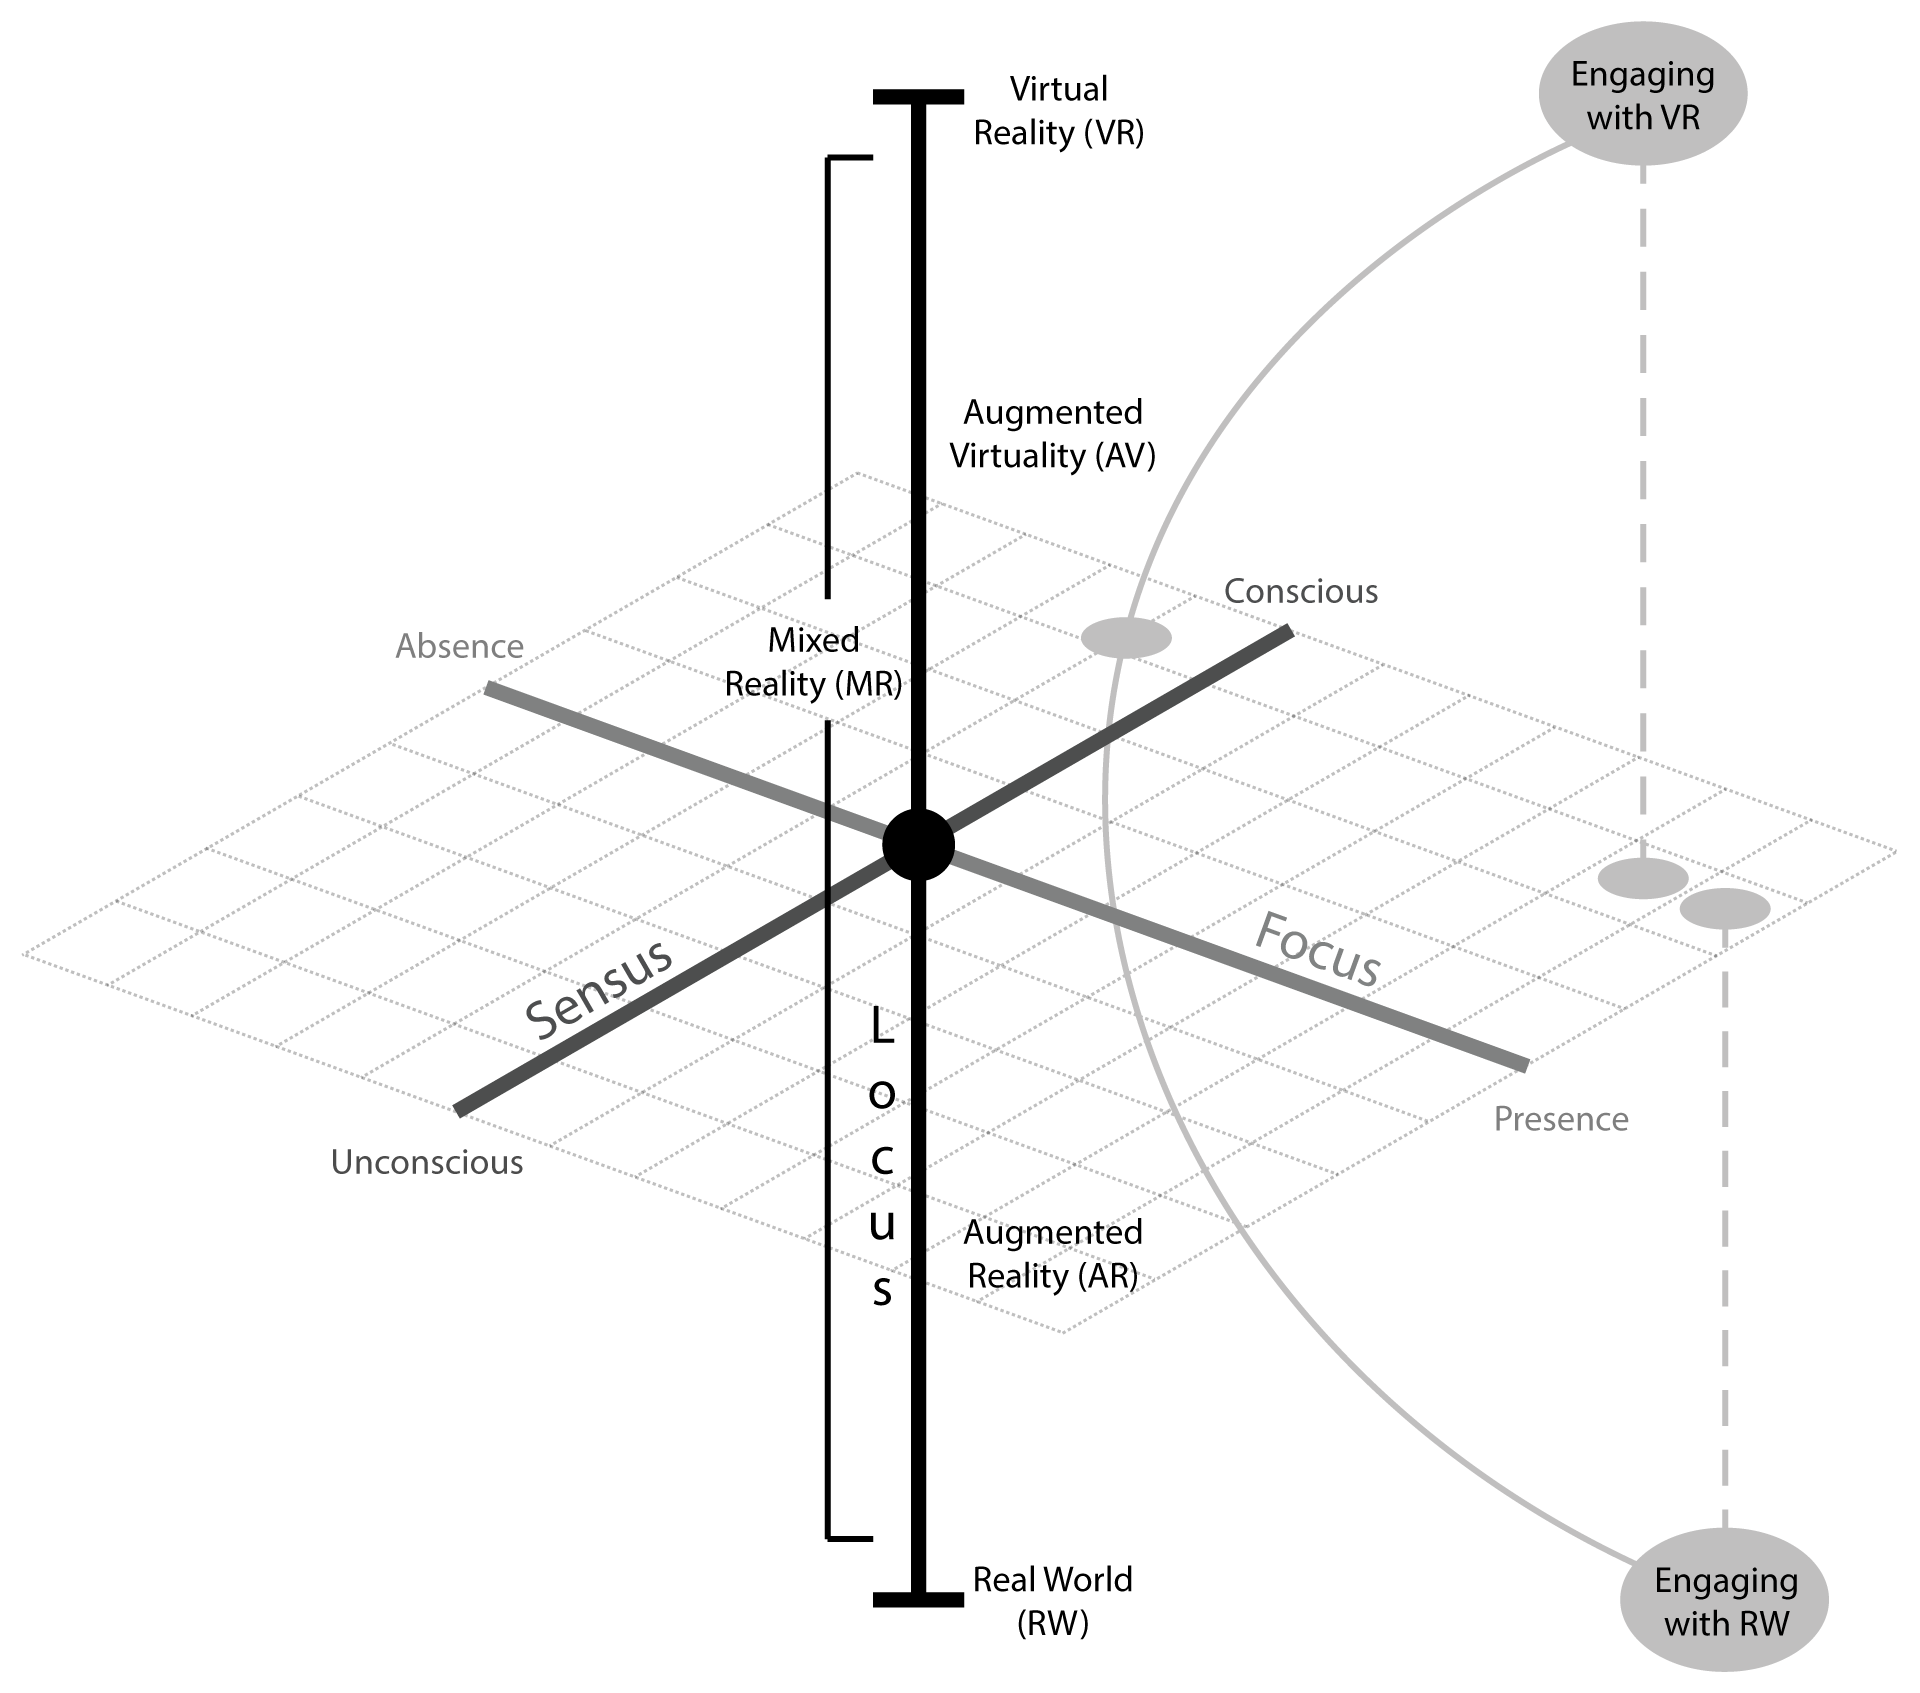
\includegraphics[width=.8\textwidth]{transition-rw-vr.png}
		\caption{Visualisation using the combined Milgram/Waterworth model of the theorised experience of a user of a PR system performing a slow transition between its constituent RW and VR environments.}
		\label{focus-locus-sensus-with-virtuality-continuum-with-transition}
	\end{center}	
\end{figure}

%=========================================================================================================
%=========================================================================================================


%=========================================================================================================
%=========================================================================================================
%=========================================================================================================
%=========================================================================================================
%=========================================================================================================
%=========================================================================================================
%=========================================================================================================
%=========================================================================================================
%=========================================================================================================
%=========================================================================================================


%Users are free to explore and interact with either environment in relative isolation from the other, even if their interactions in one trigger changes in the other, however simultaneous interaction and exploration with both environments has largely remained without systematic investigation.

%This is largely because users exploring and interacting with the real environment do not have a convenient manner of also exploring and directly interacting with the virtual environment, as such interaction usually relies upon the use of software run on a desktop or laptop computer which is not conducive to mobile use. Using a laptop computer whilst walking around is far from convenient and using a desktop computer obviously limits the user's interaction with the real environment to that immediately around the location of the  computer and results in a disjoint relationship between their physical position in the real environment and the location of their avatar in the virtual environment when they navigate their avatar away from the respective position of their computer. This situation has been called `the vacancy problem'; an apparent vacancy from one environment whilst engrossed in the other.




%=========================================================================================================
%=========================================================================================================





%=========================================================================================================

%Marie Kim et al at The Electronics and Telecommunications Research Institute, Korea, explain the cross reality paradigm well in terms of its principle features

%\begin{quote}
%\textit{``The important point of X-reality is a paradigm shift from single-directional information flows to bidirectional information flows between two worlds.''}
%\end{quote}

%and also how it can be employed for simultaneous presence in real and virtual environments

%\begin{quote}
%\textit{``The differential characteristic of X-reality is that it can augment user's engagement in the experiences of virtual presence and virtual world. Ultimately, it results in the human life span extension from the only real world to both worlds.''}
%\end{quote}





%Paradiso in IEEE Pervasive, Cross Reality Environments ~\cite{Paradiso2009} \textbf{***check this is the right citation***}

%\begin{quote}
%\textit{We call the ubiquitous mixed reality environment that comes from the fusion of these two technologies cross-reality. Sensor networks can tunnel dense real-world information into virtual worlds, where this data is interpreted and displayed to dispersed users. Interaction of virtual participants can incarnate into the physical world through a plenitude of diverse displays and actuators. We can envision a user's interface into this environment as an extension of human perception and interaction, augmenting our five senses well beyond the canonical ``here and now'' and redefining the meaning of presence.''}
%\end{quote}



%\begin{quote}
%\textit{``We see cross-reality precipitating when diverse and ubiquitous sensor and actuator networks meet pervasively shared online virtual worlds, where phenomena freely tunnel between real and contrived continua at a multitude of ``wormholes'' opened by densely deployed networked devices, seamlessly adapting the level of immersion to match a variable ecology of available interfaces and user context or preference.''}~\cite{Lifton2009}
%\end{quote}



%=========================================================================================================

\section{The Case for Parallel Reality}
\label{caseforpr}
%ARCHEOGUIDE makes the point that AR is good because users are not isolated/completely immersed in a synthetic world - well Mirrorshades allows uers to more fully immerse themselves in a synthetic world, but without becoming isolated in it (eg without becoming ***vacant*** from the real world)

A PR system that presents the user with the choice between visual stimuli from both its constituent environments (RW and VR) allows that user to engage with both real and virtual content in a manner that is similar to, but has a number of advantages over previous alternate reality systems, including traditional AR implementations and XR systems;

\begin{itemize}
	\item a PR system is less critical of registration (the accurate positioning/alignment) between real and virtual, as virtual objects are seen as part of a larger virtual environment instead of being rendered atop a view of the real environment~\cite{Azuma1997};
	\item a PR system can make use of existing VR content without the overhead of decanting/extracting a subset of the virtual components into an AR framework (e.g. manually selecting which objects within the VR environment are to be displayed over the RW environment);
	\item the use of a complete VR environment allows virtual content to be more encompassing and immersive, as presenting a complete VR environment allows total control over lighting, shadows, reflections, particle effects, etc. which would be difficult or impossible for an AR platform to render atop a view of a RW environment.
	\item the vacancy problem is further addressed, but instead of doing so by linking real and virtual environments by sensor and actuator infrastructure, vacancy in either environment is alleviated by furnishing users with the ability to transition between visual stimuli from each environment.
\end{itemize}

Thus, a PR platform is well suited to situations in which interaction with the visual stimuli of both real and virtual environments is required and where one or more of the following hold true;

\begin{itemize}
	\item in lieu of accurate registration between real and virtual, there is a strong focus on the virtual environment's atmosphere and immersion~\cite{deamicis:gamebased};
	\item there is existing VR content;
	\item the visual differences between real and virtual environments are so substantial that an AR system would resort to augment (\&/or diminish) almost the whole RW view. While AR \textit{``smears an informational coating over real space''}~\cite{Andersen}, PR presents a complete virtual environment. AR is beneficial where one wishes the juxtaposition of virtual objects upon what is already present in the RW environment, however PR is better suited to situations where one wishes to present a complete virtual alternative.
\end{itemize}

%=========================================================================================================

\section{Summary}
Decades of research into alternate realities has furnished us with a rich continuum of approaches and technologies for creating, combining, augmenting and diminishing real and virtual environments. Many of the alternate reality labels that are now becoming commonplace are concerned with presenting a different environment to the user's real surroundings (as in telepresence and virtual reality) or mixing additional information into the user's view of their real or virtual surroundings (as in augmented reality and augmented virtuality).

Although less thoroughly investigated, the concept of creating an alternate reality system by combining two environments, one real and the other virtual and both complete unto themselves, into a cross reality system presents an interesting avenue for furthering alternate reality techniques and applications, in particular to addressing the vacancy problem that affects users when trying to distribute their attention between two environments. Previous cross reality research focussed on alleviating this vacancy problem by integrating sensor and actuator infrastructure into the constituent real and virtual environments of a system, such that actions and events in one environment could manifest into the other. However directly visually engaging with both environments was not often possible in these systems and only from predetermined, static locations.

This thesis introduces parallel reality as a new category of alternate reality that allows its user to visually engage with both a real and a virtual environment, transitioning between them at any point, whilst maintaining mobility to walk through the environments in tandem. In trading the sensor/actuator infrastructure of a cross reality system for direct visual engagement with both environments, the parallel reality concept further addresses the vacancy problem by providing \textit{``the means to be in more than one place (reality) at a time''}\cite{Lifton2007a}.